\documentclass[
  a4paper,
  11pt,
]{scrartcl}

\usepackage{cmap}
\usepackage[T1]{fontenc}
\usepackage[utf8]{inputenc}

\usepackage[
  cm,
  headings
]{fullpage}
\usepackage[ngerman]{babel}
\usepackage{amsmath}
\usepackage{amssymb}
% Für die Klammern der Interpretationsabbildung:
\usepackage{stmaryrd}

\usepackage{color}
\definecolor{mygray}{rgb}{0.5,0.5,0.5}
\definecolor{myblue}{rgb}{0,0,0.8}
\definecolor{myred}{rgb}{0.8,0,0}
\definecolor{mygreen}{rgb}{0,0.6,0}

\usepackage[
  colorlinks=true,
  linkcolor=myblue,
]{hyperref}

% Coole Zeichnungen:
\usepackage{tikz}
\tikzstyle{vertex}=[draw, circle, minimum size=20pt]
\tikzstyle{edge}=[draw, -]
\usetikzlibrary{%
  %backgrounds,
  %mindmap,
  %shapes.geometric,
  %shapes.symbols,
  %shapes.misc,
  %shapes.multipart,
  positioning,
  %fit,
  %calc,
  %arrows,
  automata,
  %trees,
  %decorations.pathreplacing,
}

\usepackage{pgfplots}

% Für Zeilenumbrüche ohne Indentations
\setlength{\parindent}{0pt}

\usepackage{listings}
\lstset{%
  basicstyle=\ttfamily,
  keywordstyle=\color{blue},
  commentstyle=\color{mygray},
  language=C,
  showstringspaces=false,
}

\usepackage{enumerate}
% Schönere Tabellen
% dazu gibt’s neue Kommandos:
% - \toprule[(Dicke)], \midrule[(Dicke)], \bottomrule[(Dicke)]
% - \addlinespace: Extrahöhe zwischen Zeilen
\usepackage{booktabs}
% um in Tabellen eine Zelle über mehrere Zeilen laufen zu lassen:
\usepackage{multirow}

\usepackage{algorithmic}
\renewcommand{\algorithmicrequire}{\textbf{Eingabe:}}

\usepackage{bussproofs}

% coole Kopf- und Fußzeilen:
\usepackage{fancyhdr}
% Seitenstil ist natürlich fancy:
\pagestyle{fancy}
% alle Felder löschen:
\fancyhf{}

%\fancyhead[L]{
%}
%\fancyhead[R]
%\fancyfoot[L]{}

\fancyfoot[C]{\thepage}

\title{Klausurvorbereitung: Theoretische Informatik}

\subtitle{Universität Rostock}

%\author

\date{}

\newcommand{\p}{\leq_{\textsf{p}}}
\newcommand{\N}{\mathbb{N}}
\newcommand{\Z}{\mathbb{Z}}
\renewcommand{\O}{\mathcal{O}}
\newcommand{\Ac}{\mathcal{A}}
\newcommand{\Bc}{\mathcal{B}}
\newcommand{\Cc}{\mathcal{C}}
\newcommand{\Dc}{\mathcal{D}}
\newcommand{\Kc}{\mathcal{K}}
\newcommand{\Nc}{\mathcal{N}}
\newcommand{\Rc}{\mathcal{R}}
\newcommand{\Sc}{\mathcal{S}}
\newcommand{\Tc}{\mathcal{T}}
\newcommand{\Vc}{\mathcal{V}}
\newcommand{\Zc}{\mathcal{Z}}
\renewcommand{\ae}{\leq_{\textsf{ae}}}

\newcommand{\COLOR}{\textsf{COLOR}}
\newcommand{\COLORDrei}{\textsf{COLOR-3}}
\newcommand{\DreiSAT}{\textsf{3SAT}}
\newcommand{\bin}{\text{bin}}
\newcommand{\TSP}{\textsf{TSP}}
\newcommand{\HC}{\textsf{HAMILTONIAN CIRCUIT}}
\newcommand{\TSPOPTI}{\textsf{TSP\_OPT\_1}}
\newcommand{\NELP}{\textsf{0--1 LINEAR PROGRAMMING}}
\newcommand{\CLIQUE}{\textsf{CLIQUE}}
\newcommand{\NP}{\textsf{NP}}
\newcommand{\id}{\text{id}}
\newcommand{\IS}{\textsf{INDEPENDENT SET}}
\newcommand{\VC}{\textsf{VERTEX COVER}}
\newcommand{\IV}{\textsf{INTERESSENVERTRETER}}

\newcommand{\prightarrow}{\ {}_p\!\!\rightarrow}

\begin{document}

\maketitle

\tableofcontents

\section{Themen \& Inhalte}
\label{sec:themen}

\subsection{Komplexität und formale Sprachen}
\label{sub:themen_inhalte_komplexitat_und_formale_sprachen}

\begin{itemize}
  \item \NP-Vollständigkeit durch Polynomialreduktion zeigen
    \begin{itemize}
      \item Bsp: $\DreiSAT \p \IS$
    \end{itemize}
  \item Zeigen, dass eine Sprache nicht regulär ist (Pumping-Lemma für reguläre
    Sprachen)
    \begin{itemize}
      \item Bsp: $L = \{ 0^n 1^n \mid n \in \N \}$ ist nicht regulär
    \end{itemize}
  \item Turing-Maschine bauen (deterministisch und nichtdeterministisch)
    \begin{itemize}
      \item Bsp: eine NTM mit $\Sigma = \{\Box, 0, 1\}$, die zwei Einsen auf dem
        Band erkennt (Startposition ist beliebig)
    \end{itemize}
  \item Mengenschreibweise einer Sprache aus einer gegebenen Grammatik angeben
    \begin{itemize}
      \item siehe Serie 8, Aufgabe 3 und Aufgabe 4
    \end{itemize}
  \item nicht-/deterministischen endlichen Automaten aus einer gegebenen
    Grammatik konstruieren
    \begin{itemize}
      \item siehe Serie 8, Aufgabe 3 und Aufgabe 4
      \item dazu gehört auch: eine rechtslineare Grammatik normalisieren
    \end{itemize}
  \item deterministischen endlichen Automaten minimieren
    \begin{itemize}
      \item siehe Serie 9, Aufgabe 3
      \item siehe \hyperref[sub:serie_10]{Serie 10},
        \hyperref[kfs_serie_10_aufgabe_1]{Aufgabe 1}
    \end{itemize}
  \item Pumpingzahl einer regulären Sprache angeben
    \begin{itemize}
      \item siehe \hyperref[sub:serie_10]{Serie 10},
        \hyperref[kfs_serie_10_aufgabe_2_c]{Aufgabe 2 (c)}
    \end{itemize}
  \item NDEA $\rightarrow$ DEA
    \begin{itemize}
      \item siehe Serie 9, Aufgabe 1
      \item siehe auch das Beispiel aus~\cite{hopcroft2011}:

        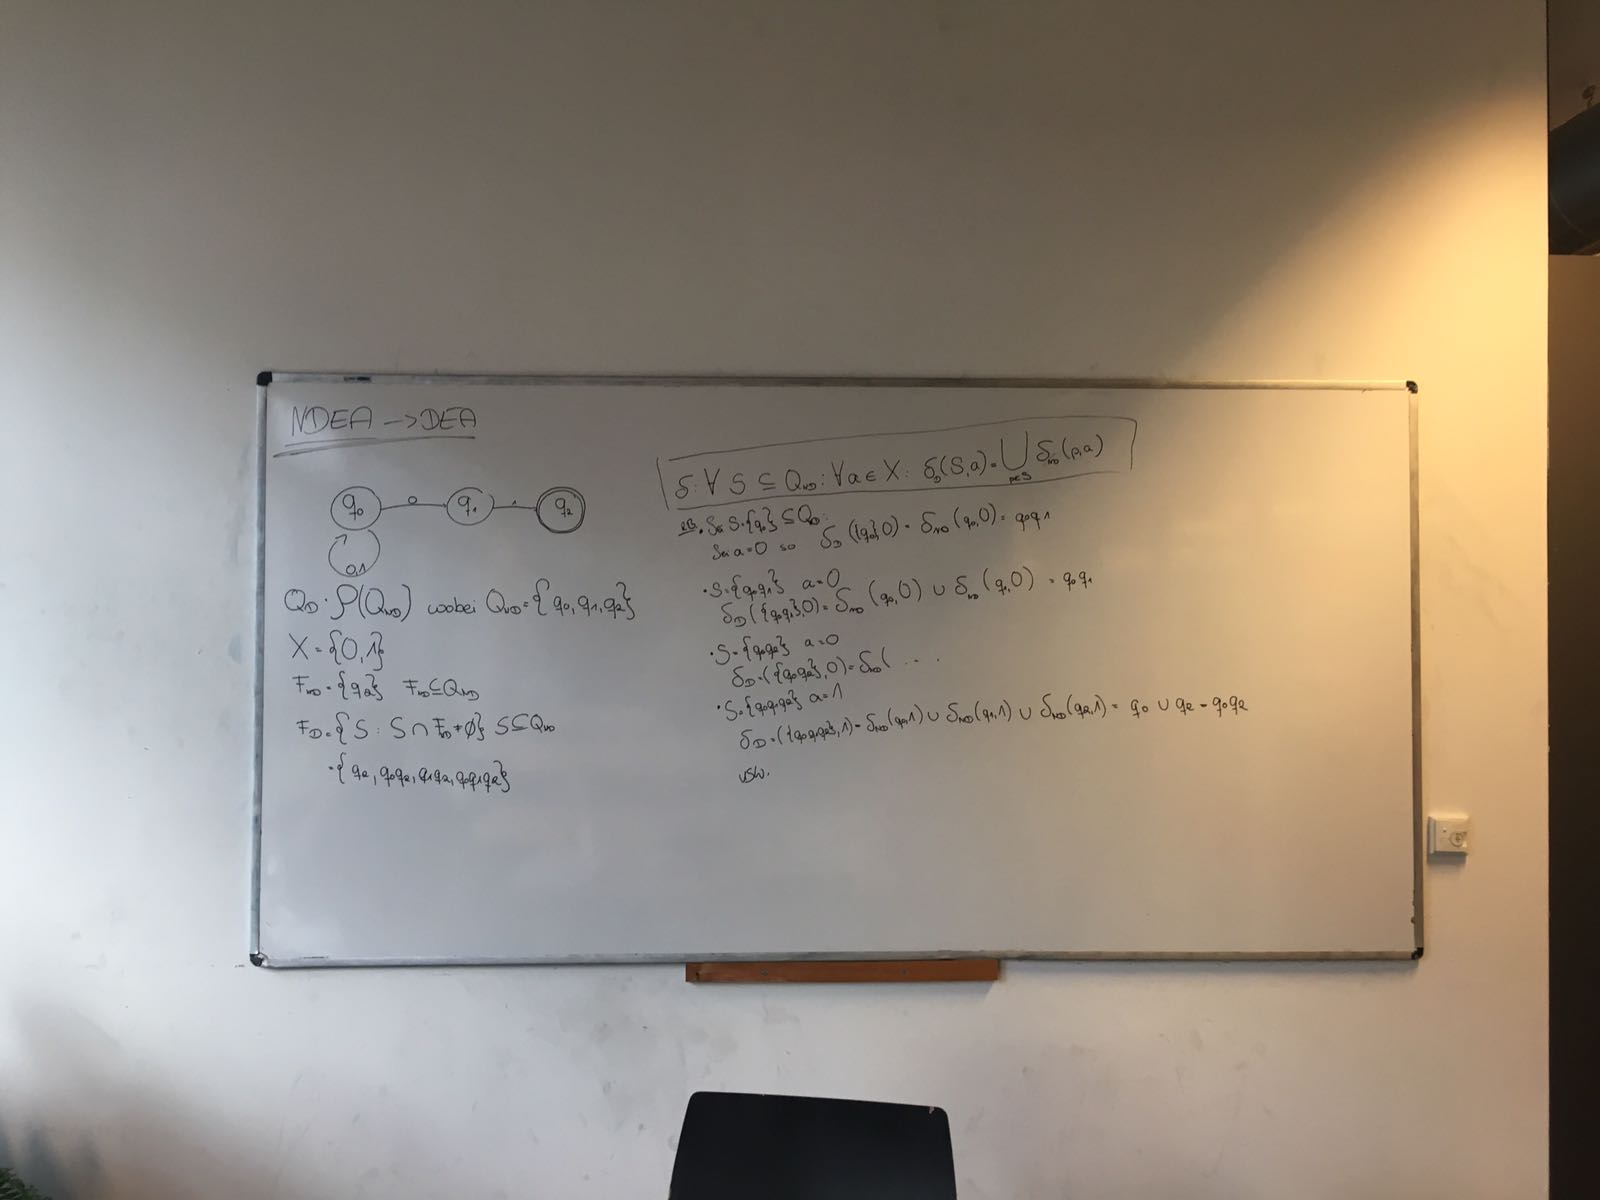
\includegraphics[width=0.9\textwidth]{bilder/ndea_zu_dea_bsp_aus_hopcroft.jpg}
    \end{itemize}
\end{itemize}

\subsection{Semantik}
\label{sub:themen_inhalte_semantik}

\subsubsection{Induktion}
\label{ssub:Induktion}

\paragraph{Strukturelle Induktion}
\label{par:strukturelle_induktion}

\begin{itemize}
  \item Bildungsregeln: eine Bildungsregel über einer beliebigen Menge $M$ ist
    ein Paar $(V, e)$ aus einer endlichen Menge $V \sqsubseteq M$, der
    sogenannten Regel-Voraussetzung, und einem Element $e \in M$, dem
    sogenannten Erzeugnis der Regel.

    Eine Regel $(\emptyset, e)$ mit leerer Regel-Voraussetzung nennen wir eine
    Verankerung. Eine Regel $(V, e)$ mit nicht-leerer Regel-Voraussetzung $V
    \neq \emptyset$ nennen wir einen Schritt.

    Die Anwendung der einzelnen Regel $(V, e)$ auf eine Teilmenge $T \subseteq
    M$ ist wieder eine Teilmenge von $M$. Sie ist definiert durch:
    \begin{align*}
      \alpha( \, (V, e), T) :=
      \begin{cases}
        \{ e \} & \text{ falls } V \subseteq T\\
        \emptyset & \text{ falls } V \subsetneq T
      \end{cases}
    \end{align*}

    Die Anwendung der Regelmenge $\Rc$ auf die Teilmenge $T$ ist wieder eine
    Teilmenge von $M$. Sie ist definiert durch:
    \begin{align*}
      \alpha_{\Rc}(T) := \bigcup\limits_{r \in \Rc} \alpha(r, T)
    \end{align*}

    Die Erweiterung der Teilmenge $T$ durch einmalige Anwendung der Regelmenge
    $\Rc$ ist gegeben durch:
    \begin{align*}
      \sigma_{\Rc}(T) := T \cup \alpha_{\Rc}(T)
    \end{align*}

    Eine Teilmenge $T \subseteq M$ heißt $\Rc$-abgeschlossen unter einer Menge
    $\Rc$ von Regeln, wenn gilt: für jede Regel $(V, e) \in \Rc$ gilt: falls die
    Voraussetzungen der Regel in der Menge $T$ enthalten sind, dann ist auch das
    Erzeugnis $e$ der Regel in der Menge $T$ enthalten:
    \begin{align*}
      \forall (V, e) \in \Rc: V \subseteq T \Rightarrow e \in T
    \end{align*}
\end{itemize}

\subsubsection{Formale Ausdrücke}
\label{ssub:formale_ausdruecke}

\paragraph{Zustände}
\label{par:zustande}

\begin{itemize}
  \item Zustände: sei \textbf{Var} eine Menge von Variablen und \textbf{Val}
    eine Menge von Werten. Ein Zustand ist eine partielle Funktion $s:
    \textbf{Var} \rightharpoonup \textbf{Val}$.

  \item Notation von Zuständen: der Zustand $s: \textbf{Var} \rightharpoonup
    \textbf{Val}$ mit $\Dc(s) = \{x_1, x_2, \dots, x_n\}$ und $s(x_i) =
    w_i$ wird auch als $[x_1 \mapsto w_1, \dots, x_n \mapsto w_n]$ notiert.

  \item Die Erweiterung des Zustands $s_1: \textbf{Var} \rightharpoonup
    \textbf{Val}$ um den Zustand $s_2: \textbf{Var} \rightharpoonup
    \textbf{Val}$ ist definiert als
    \begin{align*}
      s_1 \oplus s_1: & \textbf{Var} \rightharpoonup \textbf{Val}\\
      & v \mapsto (s_1 \oplus s_2)(v) :=
        \begin{cases}
          s_2(v), & \Leftrightarrow v \in \Dc(s_2)\\
          s_1(v), & \Leftrightarrow v \in \Dc(s_1)
            \wedge v \notin \Dc(s_2)\\
        \end{cases}
    \end{align*}

    Bei einer Erweiterung wird ein Zustand also von links nach rechts
    „überschrieben“.

    Für eine abstrakte Menge von Zuständen schreiben wir neben $\textbf{Var}
    \rightharpoonup \textbf{Val}$ gelegentlich auch $\Zc$.
\end{itemize}

\paragraph{Interpretation}
\label{par:interpretation}

\begin{itemize}
  \item Interpretationsfunktion:
    \begin{align*}
      \llbracket \ \rrbracket:
        \textbf{Exp} \rightarrow
          \Big[ \,
            \big[
              \underbrace{\textbf{Var} \rightarrow \N_0}_{\text{Zustand}}
            \big]
            \rightarrow
            \underbrace{\N_0}_{\text{Wert}}
          \Big]
    \end{align*}
    oder allgemein:
    \begin{align*}
      \llbracket \ \rrbracket:
        \textbf{Exp} \rightarrow
          \Big[ \,
            \big[
              \underbrace{\textbf{Var} \rightarrow \textbf{Val}}_{\text{Zustand}}
            \big]
            \rightarrow
            \underbrace{\textbf{Val}}_{\text{Wert}}
          \Big]
    \end{align*}
    oder:
    \begin{align*}
      \llbracket \ \rrbracket:
        \textbf{Exp} \rightarrow
          \left[\Zc \rightarrow \textbf{Val} \right]
    \end{align*}

  \item Die Interpretation eines Ausdrucks, der nur aus der Variable $x$
    besteht, ist $\llbracket x \rrbracket$. Das ist nach Definition eine
    Funktion $\left[ \textbf{Var} \rightarrow \N_0 \right] \rightarrow \N_0$.
    Für jeden Zustand $\sigma: \textbf{Var} \rightarrow \textbf{Val}$ ist somit
    $\llbracket x \rrbracket (\sigma)$ eine natürliche Zahl. Es ist naheliegend,
    hier $\llbracket x \rrbracket (\sigma) = \sigma(x)$ zu fordern: die
    Bedeutung $\llbracket x \rrbracket (\sigma)$ einer Variablen $x$ (als
    Ausdruck) in einem Zustand $\sigma$ ist durch den Wert $\sigma(x)$ der
    Variablen in diesem Zustand gegeben.
\end{itemize}

\subsubsection{Ersetzungs-Systeme}
\label{ssub:Ersetzungs-Systeme}

\paragraph{Allgemeine Ersetzungs-Systeme}
\label{par:allgemeine_ersetzungs_systeme}

\begin{itemize}
  \item Ein Ersetzungs-System (rewriting system) ist ein Paar $(M, \rightarrow)$
    bestehend aus
    \begin{enumerate}
      \item einer Menge $M$, der sogenannten Basismenge, und
      \item einer binären Relation $\rightarrow \ \subseteq M \times M$ auf $M$,
        die Reduktions-Relation genannt wird.
    \end{enumerate}
    Gilt $(a, b) \in \ \rightarrow$ so schreibt man auch $a \rightarrow b$ und
    sagt, dass $a$ zu $b$ (unmittelbar) reduziert.

  \item abgeleitete Relationen:
    \begin{itemize}
      \item transitive Reduktions-Relation
      \item reflexiv-transitive Reduktions-Relation
      \item symmetrische Reduktions-Relation
      \item symmetrisch-transitive Reduktions-Relation
      \item reflexiv-symmetrisch-transitive Reduktions-Relation
    \end{itemize}
\end{itemize}

\paragraph{Verzweigung}
\label{par:verzweigung}

\begin{itemize}
  \item endliche Verzweigung: ein Ersetzungs-System $(M, \rightarrow)$ heißt
    \begin{description}
      \item[deterministisch,] wenn es zu jedem Element höchstens einen
        unmittelbaren Nachfolger gibt. Das ist äquivalent mit der
        Rechtseindeutigkeit der Relation.
      \item[endlich verzweigt,] wenn jedes Element $a \in M$ höchstens endlich
        viele unmittelbare Nachfolger hat, d.\,h.\ die Menge $\{b \mid a
        \rightarrow b\}$ ist endlich.
    \end{description}

  \item Lemma von \textsc{König}: sei $G$ ein zusammenhängender Graph mit
    unendlich vielen Knoten. Jeder Knoten habe nur endlich viele Kanten. Dann
    ist jeder Knoten Teil eines unendlich langen, einfachen Pfads im Graph.
\end{itemize}

\paragraph{Termination}
\label{par:termination}

\begin{itemize}
  \item Terminations-Eigenschaften: sei $(M, \rightarrow)$ ein
    Ersetzungs-System. Das Element $a \in M$ heißt
    \begin{description}
      \item[irreduzibel,]  wenn es kein $b \in M$ gibt, für das $a \rightarrow
        b$ gilt.
      \item[terminierend] oder \textsc{Noether}sch, wenn es zu $a$ keine
        unendliche Kette von Reduktionen gibt, wenn es also keine $m_1, m_2,
        \dots \in M$ gibt, mit $a \rightarrow m_1 \rightarrow m_2 \rightarrow
        \dots$.
      \item[beschränkt,] wenn es eine natürliche Zahl $L$ gibt, dass jede
        Reduktionskette von $a$ eine Länge kleiner als $L$ hat.
    \end{description}

    Das Ersetzungs-System selber heißt
    \begin{description}
      \item[terminierend] oder \textsc{Noether}sch, wenn es keine unendliche
        Kette von Reduktionen gibt.
      \item[lokal beschränkt] oder in jedem Element beschränkt, wenn jedes
        Element $a \in M$ beschränkt ist.
      \item[beschränkt] oder global beschränkt, wenn es eine natürliche Zahl $L$
        gibt, sodass für jedes Element $a \in M$ jede Reduktionskette von $a$
        eine Länge kleiner als $L$ hat.
    \end{description}

  \item Terminations-Eigenschaften: für ein einzelnes Element gelten folgende
    Zusammenhänge:
    \begin{enumerate}
      \item Ist ein Element beschränkt, dann ist es auch \textsc{Noether}sch.
      \item Ist ein Element \textsc{Noether}sch, dann muss es deshalb nicht
        beschränkt sein.
    \end{enumerate}

  \item Für ein Ersetzungs-System gilt:
    \begin{align*}
      \text{Global beschränkt} \Rightarrow \text{Lokal beschränkt} \Rightarrow
      \textsc{Noether}\text{sch}
    \end{align*}

  \item Variante und Invariante: sei $(M, \rightarrow)$ ein Ersetzungs-System.
    Eine Funktion $f : M \rightarrow W$ in eine beliebige Menge $W$ heißt eine
    Invariante des Ersetzungs-Systems, wenn ihre Funktionswerte längs der
    Reduktionen invariant (= unverändert) bleibt, d.\,h.\ wenn gilt:
    \begin{align*}
      \forall x, y \in M: x \rightarrow y \Rightarrow f(x) = f(y)
    \end{align*}
    Eine Funktion $f : M \rightarrow \N$ heißt eine (abnehmende) Variante des
    Ersetzungs-Systems, wenn ihre Funktionswerte längs der Reduktionen abnehmen,
    d.\,h.\ wenn gilt:
    \begin{align*}
      \forall x, y \in M: x \rightarrow y \Rightarrow f(x) > f(y)
    \end{align*}

  \item Terminationsbeweis durch Varianten-Funktion: gibt es zu einem
    Ersetzungs-System $(S, \rightarrow)$ eine abnehmende Variante $f : S
    \rightarrow \N$, dann ist das Ersetzungs-System terminierend. Ist diese
    Variante zusätzlich als Funktion auf $S$ nach oben beschränkt, dann ist das
    Ersetzungs-System sogar (global) beschränkt.

  \item Termination endlich verzweigter Systeme: ein endlich verzweigtes
    Ersetzungs-System terminiert genau dann, wenn es lokal (also in jedem
    Element) beschränkt ist.

  \item Terminations-Hierarchie: im allgemeinen Fall sieht die Hierarchie der
    Terminations-Begriffe so aus:
    \begin{align*}
      \text{Global beschränkt} \Rightarrow \text{lokal beschränkt} \Rightarrow
      \text{terminierend}
    \end{align*}
    Für endlich verzweigte Systeme kollabiert die Hierarchie und ergibt
    \begin{align*}
      \text{Global beschränkt} \Rightarrow \text{lokal beschränkt/terminierend}
    \end{align*}
\end{itemize}

\paragraph{Konfluenz}
\label{par:konfluenz}

\begin{itemize}
  \item Konfluenz: sei $(M, \rightarrow)$ ein Ersetzungs-System. Ein Element $a
    \in M$ heißt
    \begin{description}
      \item[konfluent,] wenn für alle $b, c \in M$ mit $a \rightarrow^* b$ und
        $a \rightarrow^* c$ ein $d \in M$ existiert, für das $b \rightarrow^* d$
        und $c \rightarrow^* d$.
      \item[semi-konfluent,] wenn für alle $b, c \in M$ mit $a \rightarrow b$
        und $a \rightarrow^* c$ ein $d \in M$ existiert, für das $b
        \rightarrow^* d$ und $c \rightarrow^* d$.
      \item[lokal konfluent,] wenn für alle $b, c \in M$ mit $a \rightarrow b$
        und $a \rightarrow c$ ein $d \in M$ existiert, für das $b \rightarrow^*
        d$ und $c \rightarrow^* d$.
    \end{description}
    In allen diesen Fällen heißt $d$ ein gemeinsames Redukt von $b$ und $c$ und
    $(b,c)$ heißt ein kritisches Paar zu $a$.

    Das Ersetzungs-System $(M, \rightarrow)$ selber heißt
    \begin{description}
      \item[konfluent,] wenn jedes Element $m \in M$ konfluent ist.
      \item[semi-konfluent,] wenn jedes Element $m \in M$ semi-konfluent ist.
      \item[lokal konfluent,] wenn jedes Element $m \in M$ lokal konfluent ist.
    \end{description}

  \item Konfluenz-Eigenschaften: für jedes Ersetzungs-System $\Rc = (M,
    \rightarrow)$ gilt:
    \begin{enumerate}
      \item $\Rc$ konfluent $\Rightarrow \Rc$ semi-konfluent
        $\Rightarrow \Rc$ lokal konfluent.
      \item $\Rc$ semi-konfluent $\Rightarrow \Rc$
        konfluent.
      \item $\Rc$ lokal konfluent und terminierend $\Rightarrow
        \Rc$ semi-konfluent.
    \end{enumerate}

  \item \textsc{Church-Rosser} Eigenschaft: ein Ersetzungs-System $(M,
    \rightarrow)$ erfüllt die \textsc{Church-Rosser} Eigenschaft, wenn gilt:
    \begin{align*}
      \forall x, y \in M:
      x \leftrightarrow^* y \Rightarrow
      \exists z \in M:
      x \rightarrow^* z \wedge y \rightarrow^* z
    \end{align*}

  \item Ein Ersetzungs-System ist genau dann \textsc{Church-Rosser}, wenn es
    konfluent ist.

  \item Überblick über die Eigenschaften von Ersetzungs-Systemen:
    \begin{center}
      \begin{tabular}{c|c|c}
        Konfluenz & $\Rightarrow$ & \\
        $\Leftrightarrow$ & (immer) & \\
        Semi-Konfluenz & & Lokale Konfluenz\\
        $\Leftrightarrow$ & $\Leftarrow$ & \\
        \textsc{Church-Rosser} & (falls terminierend) &
      \end{tabular}
    \end{center}
\end{itemize}

\paragraph{Normalformen}
\label{par:normalformen}

\begin{itemize}
  \item Normalform: sei $(S, \rightarrow)$ ein Ersetzungs-System.
    \begin{itemize}
      \item Ein Element $n \in S$ heißt eine Normalform, genau dann wenn es
        irreduzibel ist.
      \item Ein Element $n \in S$ heißt eine Normalform des Elements $a \in S$,
        wenn $n$ eine Normalform ist und $a$ auf $n$ reduziert, d.\,h. $a
        \rightarrow^* n$.
      \item Das Ersetzungs-System selber heißt normalisierend, wenn es zu jedem
        Element $a \in S$ mindestens eine Normalform gibt.
      \item Ein Ersetzungs-System heißt konvergent, wenn es konfluent und
        terminierend ist.
    \end{itemize}

  \item Normalformen-Theorem:
    \begin{enumerate}
      \item \textbf{Existenz:} in einem terminierenden Ersetzungs-System $(S,
        \rightarrow)$ gibt es zu jedem Element mindestens eine Normalform.
        Anders gesagt: ein terminierendes Ersetzungs-System ist auch
        normalisierend.
      \item \textbf{Eindeutigkeit:} in einem konfluenten Ersetzungs-System $(S,
        \rightarrow)$ gibt es zu jedem Element höchstens eine Normalform. Das
        bedeutet: Normalformen sind, falls sie überhaupt existieren, eindeutig.
      \item \textbf{Existenz und Eindeutigkeit:} in einem konfluenten,
        terminierenden Ersetzungs-System gibt es zu jedem Element $s \in S$
        genau eine Normalform.
    \end{enumerate}

  \item Äquivalenz: sei $(S, \rightarrow)$ ein konvergentes Ersetzungs-System.
    Zwei Elemente $x, y \in S$ heißen äquivalent unter dem betrachteten
    Ersetzungs-System, $x \sim_{(S, \rightarrow)} y$, wenn eine der beiden
    äquivalenten Bedingungen erfüllt ist:
    \begin{enumerate}
      \item $x \leftrightarrow^* y$
      \item Die Normalform von $x$ ist gleich der Normalform von $y$.
    \end{enumerate}
\end{itemize}

\paragraph{Wort-Ersetzungs-Systeme}
\label{par:wort_ersetzungs_systeme}

\begin{itemize}
  \item Semi-\textsc{Thue} und \textsc{Thue} Systeme: ein Semi-\textsc{Thue}
    System ist ein Paar $(\Sigma, \mapsto)$ bestehend aus
    \begin{enumerate}
      \item einer endlichen Menge $\Sigma$, dem sogenannten Alphabet, und
      \item einer endlichen binären Relation $\mapsto \ \subseteq \Sigma^*
        \times \Sigma^*$ auf dem Wortmonoid von $\Sigma^*$.
    \end{enumerate}

    Ein Paar $(u, v) \in \ \mapsto$, das in Relation steht, wird auch $u \mapsto
    v$ geschrieben und heißt eine Regel des Semi-\textsc{Thue} Systems.

    Ein \textsc{Thue} System ist ein Semi-\textsc{Thue} System, dessen Relation
    symmetrisch ist.

  \item Wort-Ersetzungs-System: ein Wort-Ersetzungs-System ist ein Paar
    $(\Sigma, \rightarrow)$ bestehend aus
    \begin{enumerate}
      \item einer endlichen Menge $\Sigma$, dem sogenannten Alphabet, und
      \item einer endlichen binären Relation $\rightarrow\ \subseteq \Sigma^*
        \times \Sigma^*$ auf dem Wortmonoid von $\Sigma^*$,
    \end{enumerate}
    welche unter Anfügen beliebiger Präfixe und Postfixe in ihrer Gültigkeit
    invariant bleibt, also die folgende Eigenschaft hat:
    \begin{align*}
      \forall x,z,u,v \in \Sigma^*:
      u \rightarrow v \Rightarrow xuz \rightarrow xvz
    \end{align*}

  \item Induzierte Relationen: sei $(\Sigma, \mapsto)$ ein Semi-\textsc{Thue}
    System. Dieses induziert dann weitere Relationen auf dem Wortmonoid:
    \begin{enumerate}
      \item Die Relation der einstufigen Ableitung $\rightarrow \ \subseteq
        \Sigma^* \times \Sigma^*$ ist definiert durch die Beziehung: $a
        \rightarrow b$ genau dann, wenn $\exists x,y,u,v \in \Sigma^*$ mit
        $a = x u y, b = x v y, u \mapsto v$.

        $(\Sigma, \rightarrow)$ ist also das vom Semi-\textsc{Thue} System
        erzeugte Wort-Ersetzungs-System.

      \item Die Relation der mehrstufigen Ableitung $\rightarrow^* \ \subseteq
        \Sigma^* \times \Sigma^*$ ist definiert durch die Beziehung: $a
        \rightarrow^* b$ genau dann, wenn $\exists s_0, s_1, \dots, s_n \in
        \Sigma^*$ mit $a = s_0 \rightarrow s_1 \rightarrow \dots \rightarrow s_n
        = b$.
    \end{enumerate}

  \item Überlappungs-Eigenschaften: wir betrachten die linken Seiten $l_1, l_2$
    von den Regeln $l_1 \mapsto r_1$ und $l_2 \mapsto r_2$ eines
    Semi-\textsc{Thue} Systems. Die linken Seiten können die folgenden, für
    Konfluenz kritischen Eigenschaften aufweisen:
    \begin{description}
      \item[Gleichheit:] Die Muster der Regeln sind gleich: $l_1 = l_2$
      \item[Enthalten-Sein:] Ein Muster ist in dem anderen enthalten:
        \begin{align*}
          \exists u,v \in \Sigma^*: l_1 = u l_2 v \ \vee \ l_2 = u l_1 v
        \end{align*}
      \item[Überlappung:] Ein Muster überlappt sich mit dem anderen Muster:
        \begin{align*}
          \exists a,b,c \in \Sigma^*, b \neq \varepsilon:
          (l_1 = ab \ \wedge \ l_2 = bc) \ \vee \ (l_1 = bc \ \wedge \ l_2 = ab)
        \end{align*}
    \end{description}

  \item Echtes Enthalten-Sein: ein Muster ist in dem anderen Muster echt
    enthalten, wenn es in dem Muster enthalten ist, aber von diesem verschieden
    ist.

  \item Echte Überlappung: ein Muster überlappt sich mit dem anderen Muster
    echt, wenn es mit diesem Muster überlappt, aber von diesem verschieden ist.

  \item Kritisches Paar: die zwei Regeln $l_1 \mapsto r_1$ und $l_2 \mapsto r_2$
    bilden ein kritisches Regel-Paar, wenn das Muster einer Regel mit dem Muster
    der anderen Regel identisch ist, mit ihm echt überlappt oder in ihm echt
    enthalten ist.

  \item Konfluenz-Theorem: wir betrachten ein Wort-Ersetzungs-System, das aus
    einem Semi-\textsc{Thue} System erzeugt wird. Dann gilt: wenn die kritischen
    Paare, die sich aus den kritischen Regel-Paaren des Semi-\textsc{Thue}
    Systems ergeben, ein gemeinsames Redukt haben, dann ist das
    Wort-Ersetzungs-System lokal konfluent.
\end{itemize}

\paragraph{Term-Ersetzungs-Systeme}
\label{par:term_ersetzungs_systeme}

\begin{itemize}
  \item Term-Ersetzungs-System: sei \textbf{Exp} eine Menge von Termen über
    einer Signatur $\Tc$ und einer Variablenmenge $\Vc$.

    Ein Term-Ersetzungs-System ist eine binäre Relation $\rightarrow \ \subseteq
    \textbf{Exp} \times \textbf{Exp}$, die unter Kontext-Anwendung und unter
    Substitutions-Anwendung abgeschlossen ist.

    Das bedeutet konkret:
    \begin{enumerate}
      \item Abgeschlossen unter Kontext: für jeden Kontext ${k[]}_p$, der zu einem
        Term $k$ an einer seiner Positionen $p$ gebildet werden kann, und für
        zwei Terme $t, u$ gilt:
        \begin{align*}
          t \rightarrow u \Rightarrow {k[t]}_p \rightarrow {k[u]}_p
        \end{align*}

      \item Abgeschlossen unter Substitution: für jede Substitution $\sigma$ und
        zwei Terme $t, u$ gilt:
        \begin{align*}
          t \rightarrow u \Rightarrow \sigma(t) \rightarrow \sigma(u)
        \end{align*}
    \end{enumerate}

  \item Von Regeln erzeugte Term-Ersetzungs-Systeme: sei \textbf{Exp} eine Menge
    von Termen. Für $i = 1, \dots, n$ seien die Regeln $l_i \mapsto r_i$
    vorgegeben, genauer gesagt: es ist eine endliche Relation $\mapsto \
    \subseteq \textbf{Exp} \times \textbf{Exp}$ vorgegeben. Das von der Relation
    $\mapsto$ erzeugte Term-Ersetzungs-System $\rightarrow \ \subseteq
    \textbf{Exp} \times \textbf{Exp}$ ist nun durch einen der folgenden
    äquivalenten Ansätze definiert:
    \begin{enumerate}
      \item $\rightarrow$ ist das Kleinste aller Term-Ersetzungs-Systeme
        $\Gamma$, in denen für jedes $i$ die Reduktion $l_i \Gamma r_i$ gilt.

      \item $\rightarrow$ ist der Durchschnitt aller Term-Ersetzungs-Systeme
        $\Gamma$, in denen für jedes $i$ die Reduktion $l_i \Gamma r_i$ gilt.

      \item $v \rightarrow w$ gelte genau dann, wenn es eine Substitution
        $\sigma$ gibt, eine Regel $l = l_i \mapsto r_i = r$ und eine Position
        $p$ zum Term $v$, so dass gilt:
        \begin{align*}
          {v |}_p = \sigma(l) \qquad w = {v[\sigma(r)]}_p
        \end{align*}
    \end{enumerate}

    Theoretische Vorgehensweise:
    \begin{enumerate}
      \item Suche einen Teilterm ${v |}_p$ des Ausgangsterms $v$. Auf diesen
        Teilterm soll die Regel $l \mapsto r$ angewendet werden.

      \item Unifiziere die linke Seite $l$ der Regel durch die Substitution
        $\sigma$ mit dem Teilterm ${v |}_p$ des Ausgangsterms $\sigma(l) = {v
        |}_p$.

      \item Wende die Regeln an durch Auswertung der Substitution $\sigma$ auf
        die Regel $l \mapsto r$. Es ergibt sich die Reduktion ${v |}_p =
        \sigma(l) \rightarrow \sigma(r)$.

      \item Bette die Anwendung ein in den ursprünglichen Kontext. Wende dafür
        den Kontext ${v[]}_p$ oberhalb des Teilterms ${v |}_p$ auf beiden Seiten
        an. Es ergibt sich ${v[\sigma(l)]}_p \rightarrow {v[\sigma(r)]}_p$.
    \end{enumerate}

  \item Terminations-Lemma: für ein terminierendes Term-Ersetzungs-System
    $\rightarrow \ \subseteq \textbf{Exp} \times \textbf{Exp}$ gilt:
    \begin{enumerate}
      \item Die linke Seite einer Reduktion besteht niemals nur aus einer
        Variablen.
      \item Eine Reduktion führt keine neuen (auf der linken Seite noch nicht
        benutzten) Variablen ein. Genauer: bezeichnet $\textbf{Var}(t)$ die
        Menge der Variablen, die in einem Term auftreten und ist $t \rightarrow
        u$, dann gilt $\textbf{Var}(t) \supseteq \textbf{Var}(u)$.
    \end{enumerate}

  \item Kritisches Paar: ein kritisches Paar zu zwei Regeln $l \mapsto r$ und $s
    \mapsto t$ ist ein Paar von Termen, das auf die folgende Weise erhalten
    werden kann:
    \begin{enumerate}
      \item Trennung der Variablen: forme die Regeln so zu neuen Regeln um, dass
        die Variablenmengen der Regeln disjunkt sind. Das gelingt immer, da
        Regeln unter Substitution abgeschlossen sind.

      \item Nicht-variabler Teilterm: suche einen beliebigen (echten oder
        unechten) Teilterm ${s|}_p$ der linken Seite der einen Regel $s$, der
        aber keine Variable ist.

      \item Unifikation: bestimme den allgemeinsten Unifikator dieses Teilterms
        ${s|}_p$ und der linken Seite $l$ der anderen Regel. Dieser ist also
        eine Substitution $\sigma$ mit $\sigma(l) = \sigma({s|}_p)$.

      \item Regelanwendung: nun sind beide Regeln auf den Term $\sigma(s)$
        anwendbar und können unterschiedliche Ergebnisse liefern. Konkret:
        \begin{enumerate}
          \item Die Regel $s \mapsto t$ ist auf den Term $\sigma(s)$ direkt
            anwendbar. Sie macht daraus den Term $\sigma(t)$.

          \item Die Regel $l \mapsto r$ ist auf den entsprechenden Teilterm
            $\sigma({s|}_p)$ anwendbar, da dieser wegen $\sigma(l) =
            \sigma({s|}_p)$ mit dem Muster der Regel unifiziert werden kann. Die
            Regel macht aus dem Teilterm selber $\sigma(r)$. Der äußere Kontext
            $\sigma({s[\cdot]}_p)$ darf darauf angewendet werden und ergibt
            $(\sigma(s)){[\sigma(r)]}_p$.
        \end{enumerate}
    \end{enumerate}

    Das Paar $(\sigma(t), (\sigma(s)){[\sigma(r)]}_p$, das man auf diese Art und
    Weise aus den Regeln $l \mapsto r$ und $s \mapsto t$ erhält, heißt ein
    kritisches Paar dieser beiden Regeln.

  \item Critical Pair Lemma (\textsc{Huet}): Ein von einer Menge von Regeln
    erzeugtes Term-Ersetzungs-System ist lokal konfluent genau dann, wenn jedes
    kritische Paar $(p, q)$ der Regelmenge geschlossen werden kann, es also (in
    mehreren Schritten) zu einem gemeinsamen Term reduziert: $p \rightarrow^* z$
    und $q \rightarrow^* z$.

  \item Lineare Terme: ein Term $p \in \textbf{Exp}$ heißt linear, wenn keine
    Variable mehr als einmal in dem Term auftaucht.

    Ein Term-Ersetzungs-System heißt links-linear, wenn es aus einer Menge von
    Reduktionsregeln erzeugt werden kann, bei der die linke Seite jeder Regel
    ein linearer Term ist.

  \item Orthogonal: ein Term-Ersetzungs-System heißt orthogonal, wenn es frei
    von kritischen Paaren und links-linear ist.

  \item Satz von \textsc{Rosen}: jedes orthogonale Term-Ersetzungs-System ist
    konfluent.
\end{itemize}

\paragraph{Rekursion, Reduktion, Evaluation}
\label{par:rekursion_reduktion_evaluation}

\begin{itemize}
  \item Reduktions-Strategie: sei $(\rightarrow, \textbf{Exp})$ ein
    Term-Ersetzungs-System.

    Eine (einschrittige) Reduktions-Strategie für $\rightarrow$ ist eine
    Abbildung $\rho: \textbf{Exp} \rightarrow \textbf{Exp}$, bei der für jeden
    Term $t \in \textbf{Exp}$ gilt:
    \begin{enumerate}
      \item Falls $t$ Normalform ist, dann gilt $\rho(t) = t$
      \item In allen anderen Fällen gilt $t \rightarrow \rho(t)$.
    \end{enumerate}

    Eine (mehrschrittige) Reduktions-Strategie für $\rightarrow$ ist eine
    Abbildung $\rho: \textbf{Exp} \rightarrow \textbf{Exp}$, bei der für jeden
    Term $t \in \textbf{Exp}$ gilt:
    \begin{enumerate}
      \item Falls $t$ Normalform ist, dann gilt $\rho(t) = t$
      \item In allen anderen Fällen gilt $t \rightarrow^+ \rho(t)$.
    \end{enumerate}

  \item Redex: sei $u \rightarrow v$ eine Reduktion im Term-Ersetzungs-System
    $\rightarrow \ \subseteq \textbf{Exp} \times \textbf{Exp}$.

    Die Position $p$ im Term $u$ heißt ein Redex der Reduktion $u \rightarrow
    v$, falls $u \prightarrow w$ und $v = u{[w]}_p$. Das bedeutet anschaulich,
    dass $u$ in der Position $p$ reduzierbar ist und $v$ aus $u$ gerade durch
    eine Reduktion des Teilterms an dieser Position entsteht.

    Die Position $p$ in $u$ heißt reduzierbar, wenn es eine Reduktion $u
    \rightarrow v$ gibt, in der $p$ ein Redex dieser Reduktion ist.

    Ein Redex heißt minimal, wenn es keine reduzierbaren (echten) Teilterme
    enthält.

    Ein Redex heißt maximal, wenn es nicht (echter) Teilterm eines reduzierbaren
    Terms ist.

  \item Wichtige einschrittige Strategien: eine einschrittige
    Reduktions-Strategie $\rho : \textbf{Exp} \rightarrow \textbf{Exp}$ für ein
    Term-Ersetzungs-System $\rightarrow \ \subseteq \textbf{Exp} \times
    \textbf{Exp}$ heißt
    \begin{description}
      \item[innermost,] wenn es zu jeder Reduktion $t \rightarrow \rho(t)$ die
        Möglichkeit gibt, diese als Reduktion eines minimalen Redex zu
        interpretieren.

      \item[outermost,] wenn es zu jeder Reduktion $t \rightarrow \rho(t)$ die
        Möglichkeit gibt, diese als Reduktion eines maximalen Redex zu
        interpretieren.
    \end{description}

    Zwei spezifische Familien einschrittiger Reduktions-Strategien sind
    besonders wichtig:
    \begin{description}
      \item[leftmost innermost Reduktions-Strategien] reduzieren stets die
        linkeste reduzierbare Position, die selber keine reduzierbaren Teilterme
        mehr enthält.
      \item[leftmost outermost Reduktions-Strategien] reduzieren stets die
        linkeste reduzierbare Position.
    \end{description}

  \item Wichtige mehrschrittige Strategien:
    \begin{description}
      \item[parallel innermost Reduktions-Strategien] reduzieren simultan alle
        reduzierbaren Terme, die selber keine reduzierbaren Terme enthalten

        Beispiel: $g(f(f(0, \underline{f}(0, 1)), f(\underline{f}(2, 0),
        \underline{f}(3,1))))$ bei einem Term-Ersetzungs-System, das durch
        Regeln der Form $f(x,y) \mapsto \dots$ erzeugt wird.

      \item[parallel outermost Reduktions-Strategien] reduzieren simultan alle
        reduzierbaren Terme, die nicht Teilterm eines reduzierbaren Terms sind.

        Beispiel: $g(\underline{f}(0, f(0, 1)), \underline{f}(f(2, 0), f(3,1)))$
        bei einem Term-Ersetzungs-System, das durch Regeln der Form $f(x,y)
        \mapsto \dots$ erzeugt wird.

      \item[free argument Reduktions-Strategien] reduzieren simultan alle
        reduzierbaren Terme, bei denen zumindest ein Teilterm nicht reduzierbar
        ist.

        Beispiel: $g(\underline{f}(0, \underline{f}(0, 1)), f(\underline{f}(2,
        0), \underline{f}(3,1)))$ bei einem Term-Ersetzungs-System, das durch
        Regeln der Form $f(x,y) \mapsto \dots$ erzeugt wird.

      \item[full substitution Reduktions-Strategien] reduzieren simultan alle
        reduzierbaren Terme.

        Beispiel: $g(\underline{f}(0, \underline{f}(0, 1)),
        \underline{f}(\underline{f}(2, 0), \underline{f}(3,1)))$ bei einem
        Term-Ersetzungs-System, das durch Regeln der Form $f(x,y) \mapsto \dots$
        erzeugt wird.
    \end{description}

  \item Eigenschaften von Reduktions-Strategien: sei $\rightarrow \subseteq
    \textbf{Exp} \times \textbf{Exp}$ ein Term-Ersetzungs-System. Die (ein- oder
    mehrschrittige) Reduktions-Strategie $\rho: \textbf{Exp} \rightarrow
    \textbf{Exp}$ heißt normalisierend, wenn für jeden Term $t \in
    \textbf{Exp}$, zu dem (mindestens) eine Normalform existiert, die Folge $t,
    \rho(t), \rho^2(t), \dots$ (mindestens) eine Normalform enthält.

  \item Normalisierende Strategien: parallel outermost und full substitution
    sind für orthogonale Systeme normalisierend.

  \item Evaluation von Funktionen:
    \begin{description}
      \item[strikte Auswertung (strict evaluation)] bedeutet: bevor mit der
        Auswertung eines funktionalen Ausdrucks begonnen wird, sind die Werte
        aller Teilausdrücke zu bestimmen. Das gilt selbst dann, wenn diese
        Teilausdrücke in der Berechnung des Ausdrucks gar nicht „benötigt“
        werden.

      \item[nicht-strikte, verzögerte Auswertung (delayed evaluation)] fordert:
        die Werte der Argumente einer Funktion, werden erst dann bestimmt, wenn
        diese Argument in der Berechnung der Funktion „tatsächlich benötigt“
        wird. Dabei regelt die Semantik der spezifischen Programmiersprache, was
        mit „tatsächlich benötigt“ genau gemeint ist.

        Verzögerte Auswertung erlaubt die Beschreibung etlicher unendlicher
        Datenstrukturen, da diese erst dann (teilweise) aufgebaut werden, sobald
        die entsprechenden Komponenten benötigt werden. Die unendliche Struktur
        wird also nicht tatsächlich, sondern nur virtuell aufgebaut.
    \end{description}

  \item Strikte und verzögerte Auswertung ist eine Eigenschaft der Auswertung
    einer Funktionsbeschreibung und keine Eigenschaft der Funktion selbst.
\end{itemize}

\subsubsection{Semantik einfacher Sprachen}
\label{ssub:Semantik einfacher Sprachen}

\paragraph{Die Schleifensprache LOOP}
\label{par:die_schleifensprache_loop}

\begin{itemize}
  \item Grammatik von \textsc{Loop}:
    \begin{align*}
      \texttt{<Aexp>} \quad \rightarrow \quad
        & \texttt{<Num> | <Var> |}\\
        & \texttt{(<Aexp> + <Aexp>) | (<Aexp> - <Aexp>) |}\\
        & \texttt{(<Aexp> * <Aexp>)}\\
      \texttt{<Bexp>} \quad \rightarrow \quad
        & \texttt{T | F |}\\
        & \texttt{(<Aexp> = <Aexp>) | (<Aexp> <= <Aexp>) |}\\
        & \texttt{(<Bexp> AND <Bexp>) | (<Bexp> OR <Bexp>) |}\\
        & \texttt{NOT (<Bexp>)}\\
      \texttt{<Stm>} \quad \rightarrow \quad
        & \texttt{<Var> := <Aexp> |}\\
        & \texttt{SKIP |}\\
        & \texttt{( <Stm> ; <Stm> ) |}\\
        & \texttt{IF <Bexp> THEN <Stm> ELSE <Stm> FI |}\\
        & \texttt{LOOP <Aexp> DO <Stm> OD}\\
    \end{align*}

  \item Semantik der Sprache \textsc{Loop}:
    aus Sicht der formalen Sprachen ist dies eine kontextfreie Grammatik mit den
    Nichtterminalen \texttt{<Aexp>}, \texttt{<Bexp>}, \texttt{<Stm>},
    \texttt{<Num>} und \texttt{<Var>}. Uns interessieren jetzt jedoch nicht die
    syntaktischen Aspekte der Sprache, sondern die semantischen (also welche
    Bedeutung wir den einzelnen Elementen der Sprache zuschreiben).

    Die Nichtterminale führen uns zu fünf syntaktischen Kategorien, für die
    jeweils eine Interpretation angegeben werden soll:
    \begin{itemize}
      \item Variablensymbole
      \item Konstantensymbole
      \item \textsc{Bool}sche Ausdrücke
      \item arithmetische Ausdrücke
      \item Anweisungen (bzw. Statements)
    \end{itemize}

    Im Abschnitt~\nameref{par:zustande} (\ref{par:zustande}) haben wir schon den
    Ansatz über die Interpretation von Variablen kennengelernt. Daraus ergibt
    sich:
    \begin{align*}
      \llbracket \ \rrbracket_{\Vc}: \quad
        \textbf{Var} \rightarrow
          \big[
            \left[ \textbf{Var} \rightarrow \Z \right]
            \rightarrow \Z
          \big]
    \end{align*}
    Die Interpretation numerischer Konstanten kann man einfach oder konsistent
    mit den anderen Interpretationen festlegen:
    \begin{align*}
      \llbracket \ \rrbracket_{\Nc}: \quad &
        \textbf{Num} \rightarrow \Z\\
      \llbracket \ \rrbracket_{\Nc}: \quad &
        \textbf{Num} \rightarrow
          \big[
            \left[ \textbf{Var} \rightarrow \Z \right]
            \rightarrow \Z
          \big]
    \end{align*}
    Analog folgt die Interpretation für \textsc{Bool}sche und arithmetische
    Ausdrücke:
    \begin{align*}
      \llbracket \ \rrbracket_{\Bc}: \quad &
        \textbf{Bexp} \rightarrow
          \big[
            \left[ \textbf{Var} \rightarrow \Z \right]
            \rightarrow \{ \textbf{T}, \textbf{F} \}
          \big]\\
      \llbracket \ \rrbracket_{\Ac}: \quad &
        \textbf{Aexp} \rightarrow
          \big[
            \left[ \textbf{Var} \rightarrow \Z \right]
            \rightarrow \Z
          \big]\\
    \end{align*}
    Anweisungen werden den jeweiligen Zustand verändern und bekommen daher am
    besten die Interpretation als Zustandstransformator:
    \begin{align*}
      \llbracket \ \rrbracket_{\Sc}: \quad &
        \textbf{Stm} \rightarrow
          \big[
            \left[ \textbf{Var} \rightarrow \Z \right]
            \rightarrow
            \left[ \textbf{Var} \rightarrow \Z \right]
          \big]
    \end{align*}
    Mit der Konvention von $\Zc := \textbf{Var} \rightarrow \Z$ können wir das
    noch übersichtlicher schreiben:
    \begin{center}
      \begin{tabular}{lll}
        $\llbracket \ \rrbracket_{\Vc}$:
        & \textbf{Var}
        & $\rightarrow \ \left[ \Zc \rightarrow \Z \right]$\\
        $\llbracket \ \rrbracket_{\Nc}$:
        & \textbf{Num}
        & $\rightarrow \ \left[ \Zc \rightarrow \Z \right]$\\
        $\llbracket \ \rrbracket_{\Bc}$:
        & \textbf{Bexp}
        & $\rightarrow \ \left[ \Zc \rightarrow \{ \textbf{T}, \textbf{F} \} \right]$\\
        $\llbracket \ \rrbracket_{\Ac}$:
        & \textbf{Aexp}
        & $\rightarrow \ \left[ \Zc \rightarrow \Z \right]$\\
        $\llbracket \ \rrbracket_{\Sc}$:
        & \textbf{Stm}
        & $\rightarrow \ \left[ \Zc \rightarrow \Zc \right]$\\
      \end{tabular}
    \end{center}
\end{itemize}

\paragraph{Die Bedingungssprache WHILE}
\label{par:die_bedingungssprache_while}

\begin{itemize}
  \item Jetzt wird’s spannend, weil die Situation eintreten kann, dass das
    Programm nicht terminiert. Wir geben vier verschiedene (aber äquivalente)
    Semantiken an:
    \begin{description}
      \item[rekursive Semantik] beschreibt ein Programm als einen partiell
        definierten Zustandstransformator, der aus einem
        \textcolor{myred}{Anfangszustand} einen \textcolor{myblue}{Endzustand}
        macht:
        \begin{align*}
          \llbracket \ \rrbracket_{\Sc}:
          \textbf{Stm} \rightarrow
          \Big[
            \textcolor{myred}{\big[ \textbf{Var} \rightarrow \Z \big]}
            \rightharpoonup
            \textcolor{myblue}{\big[ \textbf{Var} \rightarrow \Z \big]}
          \Big]
        \end{align*}

      \item[Continuation Semantik] beschreibt ein Programm als eine totale
        Funktion, die einen \textcolor{myred}{Zustand} in einen
        \textcolor{myblue}{Zustand} und eine \textcolor{mygreen}{Continuation}
        abbildet:
        \begin{align*}
          \llbracket \ \rrbracket_{\Cc}:
          \textbf{Stm} \rightarrow
          \Big[
            \textcolor{myred}{\big[ \textbf{Var} \rightarrow \Z \big]}
            \rightarrow
            \textcolor{myblue}{\big[ \textbf{Var} \rightarrow \Z \big]}
            \times
            \textcolor{mygreen}{\textbf{Stm}}
          \Big]
        \end{align*}

      \item[natürliche Semantik] beschreibt ein Programm als eine Relation, die
        ausdrückt, wie ein Programm auf einen \textcolor{myred}{Zustand} wirkt
        und sich daraus unter Umständen ein \textcolor{myblue}{Endzustand}
        ergeben kann:
        \begin{align*}
          \rightarrow \ \subseteq
          \Big(
          \textbf{Stm}
          \times
          \textcolor{myred}{\big[ \textbf{Var} \rightarrow \Z \big]}
          \Big)
          \times
          \textcolor{myblue}{\big[ \textbf{Var} \rightarrow \Z \big]}
        \end{align*}

      \item[strukturelle Semantik] beschreibt ein Programm wie die natürliche
        Semantik, nur dass auf der rechten Seite neben einem
        \textcolor{myblue}{Zustand} auch noch eine
        \textcolor{mygreen}{Continuation} plus \textcolor{myblue}{Zustand}
        möglich ist:
        \begin{align*}
          \rightarrow \ \subseteq
          \Big(
          \textbf{Stm}
          \times
          \textcolor{myred}{\big[ \textbf{Var} \rightarrow \Z \big]}
          \Big)
          \times
          \Big(
          \textcolor{mygreen}{\textbf{Stm}}
          \times
          \textcolor{myblue}{\big[ \textbf{Var} \rightarrow \Z \big]}
          \Big)
          \cup
          \textcolor{myblue}{\big[ \textbf{Var} \rightarrow \Z \big]}
        \end{align*}
    \end{description}
\end{itemize}

\subsubsection{Denotationelle Semantik}
\label{ssub:Denotationelle Semantik}

\begin{itemize}
  \item Domain: sei $D$ eine Menge und $\sqsubseteq \subseteq D \times D$ eine
    Ordnungsrelation (reflexiv, identitiv, transitiv).

    Eine (aufsteigende) $\omega$-Kette ist eine monoton wachsende Folge von
    Elemente in $D$ (also eine Funktion $a: \N_0 \rightarrow D$ bzw. Familie
    ${(a_n)}_{n \in \N_0}$) mit
    \begin{align*}
      a_0 \sqsubseteq a_1 \sqsubseteq a_2 \sqsubseteq \dots
    \end{align*}
    Eine Kette ist eine linear geordnete Menge.

    Sei $S \subseteq D$ eine Menge. Ein Element $d \in D$ heißt eine obere
    Schranke von $S$, wenn jedes Element $s$ von $S$ kleiner ist als $d$:
    \begin{align*}
      \forall s \in S: s \sqsubseteq d
    \end{align*}

    Eine Menge $T \subseteq D$ besitzt ein kleinstes Element $s$, wenn jedes
    andere Element in $T$ größer ist als $s$ und $s$ in $T$ liegt.

    Ein Element $d \in D$ heißt die kleinste obere Schranke von $S$, wenn die
    Menge aller oberen Schranken von $S$ ein kleinstes Element besitzt.

    Ein Domain ist ein Paar $(D, \sqsubseteq)$ aus einer Menge und einer
    Ordnungsrelation mit den folgenden beiden Eigenschaften:
    \begin{enumerate}
      \item Es gibt ein kleinstes Element $\bot \in D$. Das bedeutet:
        \begin{align*}
          \exists \bot \in D:
            \forall d \in D:
              \bot \sqsubseteq d
        \end{align*}

      \item Jede Kette in $D$ besitzt eine kleinste obere Schranke in $D$.
    \end{enumerate}

    In einem Domain bezeichne $\sup\limits_{n \in \N_0}$ die kleinste obere
    Schranke einer aufsteigenden $\omega$-Kette $a_0, a_1, \dots$. Analog
    bezeichne $\sup \Kc$ die kleinste obere Schranke einer beliebigen Kette.

  \item Monotonie, Stetigkeit, Striktheit: seien $(A, \sqsubseteq_A)$ und $(B,
    \sqsubseteq_B)$ zwei Domains.

    Eine Funktion $f: A \rightarrow B$ heißt
    \begin{description}
      \item[monoton,] wenn gilt:
        \begin{align*}
          \forall a_1, a_2 \in A:
            a_1 \sqsubseteq_A a_2 \Rightarrow f(a_1) \sqsubseteq_B f(a_2)
        \end{align*}

      \item[stetig,] wenn für jede aufsteigende Kette ${(a_n)}_{n \in \N_0}$:
        \begin{align*}
          f \left( \sup\limits_{n \in \N_0} (a_n) \right)
          =
          \sup\limits_{n \in \N_0} \left( f (a_n) \right)
        \end{align*}

      \item[strikt,] wenn sie das kleinste Element des ersten Domains auf das
        kleinste Element des zweiten Domains abbildet:
        \begin{align*}
          f ( \bot_A ) = \bot_B
        \end{align*}
    \end{description}
\end{itemize}

\section{Übungsserien}

\subsection{Komplexität und Formale Sprachen}
\label{sub:komplexitat_und_formale_sprachen}

\subsubsection{Serie 1}
\label{sub:serie_1}

\begin{enumerate}
  \item
    \begin{enumerate}
      \item Die TM überprüft die \textsc{Palindrom}-Eigenschaft rekursiv, indem
        es das erste und das letzte Zeichen auf Gleichheit überprüft. Bei
        Gleichheit werden das erste und letzte Zeichen bei diesem Vorgang
        entfernt und der Vorgang beginnt erneut.

        Wörter der Länge $< 2$ sind dabei immer Palindrome.

      \item Wir betrachten das Wort $abaaba$ der Länge $n = 6$.

        Der Algorithmus der oben definierten TM arbeiten in vier „Phasen“, die
        jeweils unterschiedlich viele Schritte (Kopfbewegungen) benötigen.
        Wir nehmen an, dass der Kopf der TM zu Beginn am Anfang des Wortes
        steht.\footnote{Wir können die TM auch so verändern, dass der Kopf zu
        Beginn am Ende des Wortes oder sogar dahinter steht. Dazu müssen wir
        einfach eine zusätzliche Phase einbauen, die den Kopf zum Anfang des
        Wortes laufen lässt. Dies würde linearen Aufwand hinzufügen, was am Ende
        keinen Unterschied macht.}

        \begin{tabular}{cll}
          Phase & Beschreibung & benötigte Schritte\\
          \midrule
          I & erstes Zeichen lesen & $1$\\
          II & zum letzten Zeichen gehen & $6 = n$\\
          III & letztes Zeichen lesen & $1$\\
          IV & zum ersten Zeichen gehen & $5 = n-1$\\
          \midrule
          & & $13 = 2n+1$\\
          \bottomrule
        \end{tabular}

        Es bleibt das Wort $baab$ der Länge $4$ übrig. Der Algorithmus beginnt
        erneut und benötigt $2(n-2) + 1 = 9$ Schritte. Für das Wort $aa$ der
        Länge $2$ werden $2(n-4) + 1 = 5$ Schritte und für das leere Wort wird
        $1$ Schritt benötigt („springe in den akzeptierenden Zustand“).

        Um die Gleichheit des ersten und letzten Buchstabens eines Wortes der
        Länge $n$ zu überprüfen, werden $2n+1$ Schritte benötigt. Dies
        funktioniert auch für ein Wort der Länge $1$:

        \begin{tabular}{cll}
          Phase & Beschreibung & benötigte Schritte\\
          \midrule
          I & erstes Zeichen lesen & $1$\\
          II & zum letzten Zeichen gehen & $1$\\
          III' & in den akzeptierenden Zustand springen & $1$\\
          \midrule
          & & $3$\\
          \bottomrule
        \end{tabular}

        Die Anzahl der insgesamt benötigten Schritte berechnet sich durch
        folgende Summenformel:
        \begin{align*}
          \sum\limits_{k=0}^{\lfloor n/2 \rfloor} 2(n - 2k) + 1
        \end{align*}

        Für ein Wort der Länge $6$ werden insgesamt $13 + 9 + 5 + 1 = 28$
        Schritte benötigt.

        Die obere Grenze für den Index wird abgerundet, damit die Summation auch
        für Wörter ungerader Länge funktioniert.

        Für die genaue Abschätzung betrachten wir zunächst die Anzahl der
        Einsen. Diese beträgt $\lfloor n/2 \rfloor + 1$, da der Index bei $0$
        startet. Somit erhalten wir:
        \begin{align*}
          \sum\limits_{k=0}^{\lfloor n/2 \rfloor} 2(n - 2k) + 1
          = \lfloor n/2 \rfloor + 1 + \sum\limits_{k=0}^{\lfloor n/2 \rfloor} 2(n - 2k)
        \end{align*}

        Den konstanten Faktor $2$ können wir ohne Probleme herausziehen:
        \begin{align*}
          \lfloor n/2 \rfloor + 1 + \sum\limits_{k=0}^{\lfloor n/2 \rfloor} 2(n - 2k)
          = \lfloor n/2 \rfloor + 1 + 2 \sum\limits_{k=0}^{\lfloor n/2 \rfloor} n - 2k
        \end{align*}

        Den Term $\sum\limits_{k=0}^{\lfloor n/2 \rfloor} n - 2k$ können wir in
        zwei Summen aufspalten:
        \begin{align*}
          \lfloor n/2 \rfloor + 1 + 2 \sum\limits_{k=0}^{\lfloor n/2 \rfloor} n - 2k
          = \lfloor n/2 \rfloor + 1 + 2
            \left(
              \sum\limits_{k=0}^{\lfloor n/2 \rfloor} n
              - 2 \sum\limits_{k=0}^{\lfloor n/2 \rfloor} k
            \right)
        \end{align*}

        Der Term
        $\sum\limits_{k=0}^{\lfloor n/2 \rfloor} n$
        vereinfacht sich zu dem Produkt
        $\left( \lfloor n/2 \rfloor + 1 \right) n$
        und der Term
        $\sum\limits_{k=0}^{\lfloor n/2 \rfloor} k$
        ist die Gaußsche Summenformel, also
        $\frac{\lfloor n/2 \rfloor \left(\lfloor n/2 \rfloor + 1\right)}{2}$.

        Damit landen wir bei
        \begin{align*}
          \lfloor n/2 \rfloor + 1 + 2
            \left(
              \sum\limits_{k=0}^{\lfloor n/2 \rfloor} n
              - 2 \sum\limits_{k=0}^{\lfloor n/2 \rfloor} k
            \right)
          & = \lfloor n/2 \rfloor + 1 + 2
            \left(
              \left( \lfloor n/2 \rfloor + 1 \right) n
              - 2
              \frac{\lfloor n/2 \rfloor \left(\lfloor n/2 \rfloor + 1\right)}{2}
            \right)\\
          & = \lfloor n/2 \rfloor + 1 + 2
            \left( \lfloor n/2 \rfloor + 1 \right)
            \left( n - \lfloor n/2 \rfloor \right)
        \end{align*}

        Wir wählen für die weitere Analyse die Abschätzung
        $\lfloor n/2 \rfloor \leq \frac{n}{2}$
        und erhalten:
        \begin{align*}
          \lfloor n/2 \rfloor + 1 + 2
            \left( \lfloor n/2 \rfloor + 1 \right)
            \left( n - \lfloor n/2 \rfloor \right)
          & \leq \frac{n}{2} + 1 + 2
            \left( \frac{n}{2} + 1 \right)
            \left( n - \frac{n}{2} \right)\\
          & = \frac{1}{2} n^2 + \frac{3}{2} n + 1
            = \frac{1}{2} (n+2) (n+1)
            = \binom{n+2}{2}
        \end{align*}
        Eine kombinatorische Begründung fällt mir dafür aber nicht ein.

      \item --- % Es gilt $\frac{1}{2} n^2 + \frac{3}{2} n + 1 \in O(n^2)$.
        % Ist wohl falsch: „Laut VL: worst case des besten Programmes (??) O(n)“
        % Dabei kann ich (??) nicht entziffern.

      \item ---
    \end{enumerate}

    \item \begin{enumerate}
      \item Ist korrekt. Es ist zu zeigen, dass für fast alle $n$ und ein
        beliebiges $k \in \N \setminus \{ 0 \}$ gilt:
        \begin{align*}
          3n + 4 + \log n \leq k \cdot n
        \end{align*}
        Wir wählen $k := 5$ und erhalten:
        \begin{align*}
          3n + 4 + \log n & \leq 5n\\
          4 + \log n & \leq 2n = n + n
        \end{align*}
        Es gilt $4 \leq n$ für fast alle $n$ (nämlich ab $n > 4$).

        Bleibt zu zeigen, dass $\log n \leq n$.
        Wir wenden die $e$-Funktion auf beiden Seiten an und erhalten:
        \begin{align*}
          n \leq e^n = \sum\limits_{i=0}^{\infty} \frac{n^i}{i!} = 1 + n + \dots
        \end{align*}
        Daraus folgt $n \leq 1 + n$ für alle $n \in \N$. \hfill $\blacksquare$

      \item Ist korrekt. Es ist zu zeigen, dass für fast alle $n$ und ein
        beliebiges $k \in \N \setminus \{ 0 \}$ gilt:
        \begin{align*}
          \log n \leq k \cdot \sqrt{n}
        \end{align*}
        Wir wählen $k := 2$ und erhalten:
        \begin{align*}
          \log n & \leq 2 \sqrt{n}\\
          n & \leq e^{2 \sqrt{n}} \geq 1 + 2 \sqrt{n} + \frac{2 n}{2}\\
          n & \leq 1 + 2 \sqrt{n} + n\\
          0 & \leq 1 + 2 \sqrt{n}
        \end{align*}
        Die letzte Aussage ist für alle $n \in \N$ wahr. \hfill $\blacksquare$

      \item Ist nicht korrekt. Sei $k \in \N \setminus \{ 0 \}$ beliebig, aber
        fest gewählt.

        Es gilt
        \begin{align*}
          \sum\limits_{i = 1}^{n} i = \frac{n(n+1)}{2}
        \end{align*}
        Es wäre zu zeigen, dass für fast alle $n \in \N$ gilt:
        \begin{align*}
          \frac{n(n+1)}{2} & \leq k \cdot n\\
          n(n+1) & \leq 2k \cdot n
        \end{align*}
        Für $n > 0$ müsste gelten:
        \begin{align*}
          n+1 & \leq 2k
        \end{align*}
        Ab $n \geq 2k$ ist die Ungleichung aber nicht mehr erfüllt. Also gilt
        \begin{align*}
          \sum\limits_{i = 1}^{n} i \notin O(n)
        \end{align*}
        \ \hfill $\blacksquare$
    \end{enumerate}

    \item ---

    \item Die Komplexität des Suchalgorithmus „binäre Suche“ liegt in
      $O(\log n)$ bzw.\ genauer gesagt in $O(\log_2 n)$, da das Intervall, in
      welchem das Schlüsselement gesucht wird, bei jedem rekursiven Aufruf
      mindestens um die Hälfte verringert wird.

      Man könnte den Verlauf der binären Suche als Binärzahl interpretieren.
      Jede Stelle gibt entweder „suche links weiter“ ($0$) oder „suche rechts
      weiter“ ($1$) an. Im schlimmsten Fall wird immer nur links oder rechts
      gesucht. Falls immer nur rechts weitergesucht wird, erhalten wir die
      Binärdarstellung von $N-1$ und diese enthält $\log_2 (N-1)$ Einsen. Falls
      immer nur links weitergesucht wird, erhalten wir $\log_2 (N-1)$ Nullen.
\end{enumerate}



\subsubsection{Serie 2}
\label{sub:serie_2}

\begin{enumerate}
  \item
    \begin{enumerate}[(a)]
      \item Sei $\Sigma$ ein beliebiges nichtleeres Alphabet. Es ist $L \in P$,
        genau dann wenn $L \subseteq \Sigma^*$ und eine Turingmaschine $M$
        existiert, die die char. Funktion
        $\chi_L: \Sigma^* \rightarrow \{0, 1\}$
        in polynomieller Zeit berechnet. Im Endzustand von $M$ steht auf dem
        Band demnach:
        \begin{align*}
          M(\omega) = \begin{cases}
            1 & \omega \in L\\
            0 & \omega \notin L
          \end{cases}
        \end{align*}
        Dazu betrachten wir die Turingmaschine $M'$, die im Endzustand auf dem
        Band folgendes Ergebnis liefert:
        \begin{align*}
          M'(\omega) = \begin{cases}
            1 & M(\omega) = 0\\
            0 & M(\omega) = 1
          \end{cases}
        \end{align*}
        Die Turingmaschine $M'$ berechnet also in polynomieller Zeit, ob $\omega
        \in \Sigma^* \setminus L$ ist. Daraus folgt $P \subseteq coP$.

        Analog dazu betrachten wir $L \in coP$: es ist $L \in coP$ genau dann,
        wenn $L \subseteq \Sigma^*$ und eine Turingmaschine $M$ existiert, die die
        char. Funktion
        $\chi_L: \Sigma^* \setminus L \rightarrow \{0, 1\}$
        in polynomieller Zeit berechnet. Im Endzustand von $M$ steht auf dem
        Band demnach:
        \begin{align*}
          M(\omega) = \begin{cases}
            1 & \omega \in \Sigma^* \setminus L\\
            0 & \omega \notin \Sigma^* \setminus L
          \end{cases}
        \end{align*}
        Wir definieren $M'$ wie oben und erhalten das Ergebnis, dass $M'$ in
        polynomieller Zeit berechnet, ob $\omega \in L$ ist. Daraus folgt $coP
        \subseteq P$ und insgesamt $P = coP$.

      \item Sei $L_1 \in P$ und $L_2 \in P$. Das heißt, dass die Turingmaschinen
        $M_1$ und $M_2$ existieren, die $L_1$ bzw. $L_2$ in polynomieller Zeit
        entscheiden. Der Aufwand von $M_1$ für $L_1$ sei in $O(n^{k_1})$ und der
        Aufwand von $M_2$ für $L_2$ in $O(n^{k_2})$ (für konstante Werte $k_1$
        und $k_2$).

        Die Konkatenation $L_1 L_2$ ist wie folgt definiert:
        \begin{align*}
          L_1 L_2 = \{ \omega_1 \omega_2 \mid \omega_1 \in L_1, \omega_2 \in L_2
          \}
        \end{align*}
        Wir definieren eine Turingmaschine $M$, die $L_1 L_2$ in polynomieller
        Zeit entscheidet. Diese muss ein Eingabewort $\omega$ jedoch zunächst
        so in $\omega_1$ und $\omega_2$ aufspalten, dass $\omega_1 \in L_1$ und
        $\omega_2 \in L_2$ gilt.

        Dies erfolgt nach folgendem Pseudocode:
        \begin{algorithmic}[1]
          \REQUIRE{$\omega = a_1 a_2 \ldots a_n$}
          \FOR{$i = 0$ \textbf{to} $n$}\label{alg:schleife}
          \STATE{teile $\omega$ in $\omega_1 = a_1 \ldots a_i$ und $\omega_2 = a_{i+1} \ldots a_n$}\label{alg:aufteilung}
          \STATE{berechne Ergebnis von $M_1$ mit der Eingabe $\omega_1$}
          \STATE{berechne Ergebnis von $M_2$ mit der Eingabe $\omega_2$}
          \IF{$M_1$ und $M_2$ akzeptieren ihre Eingaben}
            \STATE{akzeptiere $\omega$}
          \ENDIF{}
          \ENDFOR{}
          \IF{keine Aufteilung von $\omega$ in $\omega_1$ und $\omega_2$ führte
          in einen akzeptierenden Zustand von $M_1$ und $M_2$}
            \STATE{lehne $\omega$ ab}
          \ENDIF{}
        \end{algorithmic}
        Bei der Aufteilung von $\omega$ in $\omega_1$ und $\omega_2$ in
        Zeile~\ref{alg:aufteilung} gilt
        $a_1 \ldots a_0 = \epsilon = a_{n+1} \ldots a_n$.

        Es bleibt zu zeigen, dass $M$ die Eingabe $\omega$ in polynomieller Zeit
        akzeptiert. Wie schon erwähnt liegt der Aufwand von $M_1$ für $L_1$ in
        $O(n^{k_1})$ und der Aufwand von $M_2$ für $L_2$ in $O(n^{k_2})$.
        Insgesamt liegt der Aufwand für einen Schleifendurchlauf in $O(n^{k_1})
        + O(n^{k_2}) = O(n^k)$ mit $k = \max(k_1, k_2)$. Dazu kommt noch der
        Aufwand für die Aufteilung von $\omega$ in $\omega_1$ und $\omega_2$.
        Die Schleife in Zeile~\ref{alg:schleife} wird dabei maximal $n+1$ mal
        durchlaufen. Das heißt, dass der Aufwand für die Entscheidung von $L_1
        L_2$ gleich $(n+1) \cdot O(n^k)$ ist und damit in $O(n^{k+1})$ liegt,
        was polynomiellem Aufwand entspricht. Es gilt also $L_1 L_2 \in P$.

      \item —
    \end{enumerate}

  \item
    \begin{enumerate}[(a)]
    \item Gegeben sei ein ungerichteter Graph $(V,E)$.

      Finde das minimale $k$, sodass man die Knoten mit $k$ Farben so färben
        kann, dass benachbarte Knoten immer verschiedene Farben haben?

    \item Gegeben sei ein ungerichteter Graph $(V,E)$ mit $V = \{v_1, \ldots,
        v_n \}$. Wir können den Graphen mit maximal $n$ Farben färben und falls
        der Graph nur einen Knoten besitzt, können wir ihn mit genau einer Farbe
        färben. Der minimale Wert für $k$ befindet sich demnach im Intervall
        $[1, n]$.

        Wir nehmen an, dass der Algorithmus $\COLOR(V, E, k)$ in
        deterministischer Polynomialzeit $p(n)$ entscheiden kann, ob der
        ungerichtete Graph $(V, E)$ mit $k$ Farben gefärbt werden kann.

        Folgender Algorithmus löst die Optimierungsvariante I von \COLOR{}:
        \begin{algorithmic}
          \REQUIRE{ein ungerichteter Graph $(V, E)$}
          \STATE{min $\leftarrow 1$}
          \STATE{max $\leftarrow |V|$}
          \WHILE{min $<$ max}
            \STATE{mid $\leftarrow \lfloor (\text{min} + \text{max})/2 \rfloor$}
            \IF{$\COLOR(V, E, \text{mid})$}
              \STATE{max $\leftarrow$ mid}
            \ELSE{}
              \STATE{min $\leftarrow$ mid}
            \ENDIF{}
          \ENDWHILE{}
          \RETURN{min}
        \end{algorithmic}

        Diese Binärschachtelung benötigt maximal
        $\lfloor \text{log}_2 \, n \rfloor + 1$
        Schritte.

        Der Graph wird auf dem Band einer Turingmaschine mit dem Bandalphabet
        $\{0, 1, \#\}$ wie folgt kodiert:
        \begin{align*}
          \underbrace{\bin(1) \# \bin(2) \# \ldots \# \bin(n)}_{\text{Knoten}}
          \# \#
          \underbrace{%
            \underbrace{\bin(1) \# \bin(2)}_{\text{Kante\ } (v_1, v_2)} \# \# \ldots
          }_{\text{Kanten}}
        \end{align*}
        Die Länge der binärkodierten Eingabe ergibt sich wie folgt:
        \begin{itemize}
          \item ein binärkodierter Knoten hat maximal die Länge
            $\bin(n) \leq \lfloor \text{log}_2\, n \rfloor + 1$
          \item davon haben wir $n$ Stück
          \item dazu kommen $n-1$ Trennzeichen zwischen den Knoten
          \item[$\Rightarrow$] maximal
            $n (\lfloor \text{log}_2\, n \rfloor + 1) + n-1
            \leq n (\lfloor \text{log}_2\, n \rfloor + 2)$
            Zeichen für die Knoten
          \item in einem Graphen existieren maximal
            $\binom{n}{2} = \frac{n (n-1)}{2}$
            Kanten
          \item eine binärkodierte Kante besteht aus $2$ Knoten, einem
            Trennzeichen zwischen den Knoten und zwei Trennzeichen vor dem
            ersten Knoten
          \item[$\Rightarrow$] maximal $\frac{n (n-1)}{2}
            \cdot \left(2
            \cdot (\lfloor \text{log}_2\, n \rfloor + 1) + 1 + 2\right)
            \leq n^2 (2 \lfloor \text{log}_2\, n \rfloor + 5)$
            Zeichen für die Kanten
        \end{itemize}
        Insgesamt liegt der Aufwand demnach in
        $O\Big(
          \big(
            n (\lfloor \text{log}_2\, n \rfloor + 2)
            + n^2 (2 \lfloor \text{log}_2\, n \rfloor + 5)
          \big) \cdot p(n)
        \Big)$, was die Polynomialzeiteigenschaft zeigt.
    \end{enumerate}

  \item
    \begin{enumerate}[(a)]
      \item Optimierungsvariante I für \TSP{}:

        Gegeben sei ein vollständiger Graph $(V, E = V \times V)$ mit
        einer Kostenfunktion $c: E \rightarrow \N$.

        Finde die minimalen Kosten einer Rundreise über alle Knoten.

      Optimierungsvariante II für \TSP{}:

        Gegeben sei ein vollständiger Graph $(V, E = V \times V)$ mit
        einer Kostenfunktion $c: E \rightarrow \N$.

        Finde die minimalen Kosten einer Rundreise über alle Knoten und einen
        Kreis über alle Knoten im Graphen, der diese Kosten erfüllt.

      \item
        \begin{enumerate}[1.]
          \item Wir nehmen an, dass der Algorithmus $\TSP(V, E, c, k)$ in
            deterministischer Polynomialzeit $q(n)$ entscheiden kann, ob in dem
            vollständigem Graphen $(V, E)$ mit der Kostenfunktion
            $c: E \rightarrow \N$ eine Rundreise über alle Knoten existiert,
            dessen Kosten $\leq k$ sind.

            Folgender Algorithmus löst die Optimierungsvariante I von \TSP{}:
            \begin{algorithmic}[1]
              \REQUIRE{ein vollständiger Graph $(V, E)$ und eine Kostenfunktion $c: E \rightarrow \N$}
              \STATE{lower $\leftarrow 0$}
              \STATE{$C \leftarrow \max\,\{c(e) \mid e \in E\}$}
              \STATE{upper $\leftarrow |V| \cdot C$}
              \WHILE{lower $<$ upper}
                \STATE{mid $\leftarrow \lfloor (\text{lower} + \text{upper})/2 \rfloor$}
                \IF{$\TSP(V, E, c, \text{mid})$}
                  \STATE{upper $\leftarrow$ mid}
                \ELSE{}
                  \STATE{lower $\leftarrow$ mid}
                \ENDIF{}
              \ENDWHILE{}
              \RETURN{lower}
            \end{algorithmic}

          \item Der Graph wird auf dem Band einer Turingmaschine mit dem
            Bandalphabet $\{0, 1, \#\}$ wie folgt kodiert:
            \begin{align*}
              \underbrace{\bin(1) \# \bin(2) \# \ldots \# \bin(n)}_{\text{Knoten}}
              \# \#
              \underbrace{%
                \underbrace{\bin(1) \# \bin(2)}_{\text{Kante\ } (v_1, v_2)}
                \#
                \underbrace{\bin(c((v_1, v_2)))}_{\text{Kosten von } (v_1, v_2)}
                \# \# \ldots
              }_{\text{Kanten}}
            \end{align*}
            Die Kodierung entspricht im Wesentlichen der von Aufgabe 2. (b), nur
            dass zu jeder Kante noch die Binärkodierung der Kostenfunktion
            hinzukommt.

            Sei $C$ der im Graphen größte angenommene Wert der Kostenfunktion.
            Ein Wert der Kostenfunktion nimmt dann maximal $\lfloor \text{log}_2
            C \rfloor + 1$ Stellen in Anspruch. Dazu kommt ein Trennzeichen pro
            Kante. Insgesamt kommen maximal $n^2 \cdot \left( \lfloor
            \text{log}_2 C \rfloor + 2 \right)$ Zeichen hinzu, sodass der
            Aufwand für die Optimierungsvariante I in
            \begin{align*}
              O\Big(
                \big(
                  n (\lfloor \text{log}_2\, n \rfloor + 2)
                  + n^2 (2 \lfloor \text{log}_2\, n \rfloor + 5)
                  + n^2 \left( \lfloor \text{log}_2 C \rfloor + 2 \right)
                \big) \cdot q(n)
              \Big)
            \end{align*}
            liegt, was die Polynomialzeiteigenschaft zeigt.
        \end{enumerate}

      \item
        \begin{enumerate}[1.]
          \item Wir nehmen an, dass der Algorithmus $\TSPOPTI(V, E, c)$ in
            deterministischer Polynomialzeit $r(n)$ in dem vollständigem Graphen
            $(V, E)$ mit der Kostenfunktion $c: E \rightarrow \N$ die minimalen
            Kosten einer Rundreise über alle Knoten berechnen kann.

            Folgender Algorithmus löst die Optimierungsvariante II von \TSP{}:
            \begin{algorithmic}[1]
              \REQUIRE{ein vollständiger Graph $(V, E)$ und eine Kostenfunktion $c: E \rightarrow \N$}
              \STATE{min $\leftarrow \TSPOPTI(V, E, c)$}
              \STATE{$U \leftarrow E$}
              \WHILE{$U \neq \emptyset$}
                \STATE{wähle $e$ aus $U$}
                \STATE{$U \leftarrow U \setminus \{ e \}$}
                \STATE{$k \leftarrow \TSPOPTI(V, E \setminus \{ e \}, c)$}
                \IF{$k =$ min}
                  \STATE{$E \leftarrow E \setminus \{ e \}$}
                \ENDIF{}
              \ENDWHILE{}
              \RETURN{$E$}
            \end{algorithmic}

          \item Dieser Algorithmus überprüft für jede Kante im Graphen, ob sie
            wichtig ist und zur Rundreise gehört oder ob die Rundreise ohne sie
            teurer würde. Am Ende bleiben nur die wichtigen Kanten übrig.

            Dabei wird jede Kante einmal überprüft (wovon maximal $n^2$
            existieren), sodass die Komplexität der Optimierungsvariante II in
            $O(n^2 \cdot r(n))$ liegt.
        \end{enumerate}
    \end{enumerate}
\end{enumerate}



\subsubsection{Serie 3}
\label{sub:serie_3}

\begin{enumerate}
  \item
    \begin{enumerate}[(a)]
      \item In der Übung wurde gezeigt, dass sich \DreiSAT{} auf das
        Halteproblem reduzieren lässt.

        Um zu zeigen, dass das Halteproblem wenigstens so schwer wie
        \COLORDrei{} ist, überführen wir \COLORDrei{} in \DreiSAT{}.

        Gegeben sei ein Graph $(V, E)$ mit $|V| = n$ und eine Menge mit drei
        Farben, die wir mit $\{1,2,3\}$ abstrahieren. Wir führen für jeden
        Knoten und jede Farbe ein Literal $v_{i, c}$ (mit $i \in \{1, \ldots,
        n\}$ und $c \in \{1,2,3\}$) ein, welches angibt, ob der Knoten mit
        dieser Farbe gefärbt wurde.

        Die aussagenlogische Formel für \DreiSAT{} ergibt sich aus zwei
        Teilformeln: $K \wedge N$

        Dabei gilt:
        \begin{itemize}
          \item $K$ sind die Bedingungen für die Färbungen der einzelnen Knoten,
          \item $N$ sind die Bedingungen für die unterschiedlichen Färbungen
            benachbarter Knoten
        \end{itemize}

        Ein einzelner Knoten darf nur mit einer Farbe gefärbt werden, also gilt:
        \begin{align*}
          K = \bigwedge\limits_{i \in \{1, \ldots, n\}}
            (v_{i, 1} \vee v_{i, 2} \vee v_{i, 3}) \wedge
            (\neg v_{i, 1} \vee \neg v_{i, 2}) \wedge
            (\neg v_{i, 1} \vee \neg v_{i, 3}) \wedge
            (\neg v_{i, 2} \vee \neg v_{i, 3})
        \end{align*}

        Weiterhin dürfen benachbarte Knoten nicht mit derselben Farbe gefärbt
        werden. Es gilt also für alle $i \in \{1, \ldots, n\}$ und
        $v_j \in N(v_i)$:
        \begin{align*}
          N = \bigwedge\limits
            (\neg v_{i, 1} \vee \neg v_{j, 1}) \wedge
            (\neg v_{i, 2} \vee \neg v_{j, 2}) \wedge
            (\neg v_{i, 3} \vee \neg v_{j, 3})
        \end{align*}

        Alle Klauseln enthalten höchstens drei Literale und die Formel $K \wedge
        N$ befindet sich in konjunktiver Normalform.

      \item Während das Halteproblem nicht entscheidbar ist, weil die
        Turingmaschine unendlich lange laufen würde, ist \COLORDrei{}
        entscheidbar, da man „nur“ endlich viele Möglichkeiten ausprobieren
        muss.
    \end{enumerate}

  \item ---

  \item
    \begin{enumerate}[(a)]
      \item Um zu zeigen, dass $\NELP{} \in NP$ ist, müssen wir zeigen, dass
        eine nichtdeterministische Turingmaschine existiert, die das Problem in
        polynomieller Zeit entscheidet.

        Angelehnt an die Vorlesung agiert die NTM nach folgendem
        Pseudoalgorithmus:
        \begin{enumerate}
          \item „rate“ ein $x \in {\{0, 1\}}^n$
          \item überprüfe $f(x_1, \ldots, x_n) \geq k$ und $Ax \leq b$
        \end{enumerate}
        Da der letzte Schritt in polynomieller Zeit ausgeführt werden kann, gilt
        die Behauptung.

      \item Gegeben sei das Problem \CLIQUE{} über dem Graphen $G = (V, E)$ mit
        $n = |V|$ und $k \in \N$. Für die Reduktion auf \NELP{} betrachten wir
        den Komplementgraph $\overline{G} = (V, V \times V \setminus E)$.

        Die Matrix $A$ ergibt sich aus der Inzidenzmatrix von $\overline{G}$:
        \begin{itemize}
          \item $A$ enthält $n$ Spalten
          \item jede Zeile von $A$ bildet eine Kante aus $\overline{G}$ ab
          \item jede Zelle von $A$ enthält eine $1$, falls der Knoten der
            jeweiligen Spalte auf der Kante liegt; ansonsten eine $0$
        \end{itemize}
        $A$ hat damit $m = \binom{n}{2} - |E|$ Zeilen und $n$ Spalten. Das $k$
        aus \CLIQUE{} ist gleich dem $k$ aus \NELP{}. $c$ ist der
        $n$-dimensionale $1$-Vektor und $b$ ist der $m$-dimensionale $1$-Vektor.

        Der Lösungsvektor $x$ gibt dann an, welche Knoten in der Clique
        enthalten sind.

      \item Die Erzeugung des Komplementgraphen benötigt maximal $\binom{n}{2} =
        \frac{n(n-1)}{2}$ Schritte und um die Matrix $A$ zu erzeugen, benötigen
        wir $n \cdot m = n \cdot \left(\frac{n(n-1)}{2} - |E|\right)$ Schritte.
        Insgesamt liegt der Aufwand in $O(n^3)$ und ist damit polynomiell.

      \item Aus
        \begin{align*}
          G = (\{1,2,3,4,5,6\}, \{12, 13, 15, 23, 25, 34, 35, 45\})
        \end{align*}
        folgt
        \begin{align*}
          \overline{G} = (\{1,2,3,4,5,6\}, \{14, 16, 24, 26, 36, 46, 56\})
        \end{align*}
        Die Matrix $A$ ist demnach
        \begin{align*}
          A & = \begin{pmatrix}
            1 & 0 & 0 & 1 & 0 & 0\\
            1 & 0 & 0 & 0 & 0 & 1\\
            0 & 1 & 0 & 1 & 0 & 0\\
            0 & 1 & 0 & 0 & 0 & 1\\
            0 & 0 & 1 & 0 & 0 & 1\\
            0 & 0 & 0 & 1 & 0 & 1\\
            0 & 0 & 0 & 0 & 1 & 1\\
          \end{pmatrix}
        \end{align*}

        Die maximale Clique hat die Größe $k = 4$ und enthält die Knoten
        $\{1,2,3,5\}$. In \NELP{} ergibt das folgende Ergebnisse:
        \begin{align*}
          Ax & = \begin{pmatrix}
            1 & 0 & 0 & 1 & 0 & 0\\
            1 & 0 & 0 & 0 & 0 & 1\\
            0 & 1 & 0 & 1 & 0 & 0\\
            0 & 1 & 0 & 0 & 0 & 1\\
            0 & 0 & 1 & 0 & 0 & 1\\
            0 & 0 & 0 & 1 & 0 & 1\\
            0 & 0 & 0 & 0 & 1 & 1\\
          \end{pmatrix}
          \begin{pmatrix}
            1\\
            1\\
            1\\
            0\\
            1\\
            0
          \end{pmatrix}
          =
          \begin{pmatrix}
            1\\
            1\\
            1\\
            1\\
            1\\
            0\\
            1
          \end{pmatrix}
          \leq
          \begin{pmatrix}
            1\\
            1\\
            1\\
            1\\
            1\\
            1\\
            1
          \end{pmatrix}
          = b
        \end{align*}
        Der optimale Zielfunktionswert ist
        \begin{align*}
          \sum\limits_{i=1}^n c_i x_i = \sum\limits_{i=1}^n x_i = 4
        \end{align*}
    \end{enumerate}
\end{enumerate}



\subsubsection{Serie 4}
\label{sub:serie_4}

\begin{enumerate}
  \item \begin{enumerate}
    \item Wir zeigen: die Relation $\p$ ist auf der Menge \NP{} ist eine
      Quasiordnung.

      Seien
      $L_1 \subseteq \Sigma_1^*,
        L_2 \subseteq \Sigma_2^*,
        L_3 \subseteq \Sigma_3^*$
      Entscheidungsprobleme und
      $L_1, L_2, L_3 \in \NP$.

      \begin{description}
        \item[reflexiv] Es gilt $L_1 \p L_1$ genau dann, wenn eine polynomiale
          berechenbare Funktion $f: \Sigma_1^* \rightarrow \Sigma_1^*$
          existiert, so dass für alle Wörter $w \in \Sigma_1^*$ die Äquivalenz
          $w \in L_1 \Leftrightarrow f(w) \in L_1$ gilt.

          Diese Äquivalenz ist für $f := \id$ erfüllt, also gilt $L_1 \p L_1$.

        \item[transitiv] Es ist zu zeigen: $L_1 \p L_2$ und $L_2 \p L_3$
          impliziert $L_1 \p L_3$.

          $L_1 \p L_2$ bedeutet, dass eine polynomiale berechenbare Funktion
          $f: \Sigma_1^* \rightarrow \Sigma_2^*$ existiert, so dass für alle
          Wörter
          $w \in \Sigma_1^*$ die Äquivalenz
          $w \in L_1 \Leftrightarrow f(w) \in L_2$ gilt.

          Analog dazu bedeutet $L_2 \p L_3$, dass eine polynomiale berechenbare
          Funktion
          $g: \Sigma_2^* \rightarrow \Sigma_3^*$
          existiert, so dass für alle Wörter
          $w \in \Sigma_2^*$ die Äquivalenz
          $w \in L_2 \Leftrightarrow g(w) \in L_3$ gilt.

          Damit $L_1 \p L_3$ gilt, muss eine polynomiale berechenbare Funktion
          $h: \Sigma_1^* \rightarrow \Sigma_3^*$
          existieren, so dass für alle Wörter
          $w \in \Sigma_1^*$ die Äquivalenz
          $w \in L_1 \Leftrightarrow h(w) \in L_3$ gilt.

          Wir wählen $h := g \circ f$ und erhalten
          \begin{align*}
            w \in \Sigma_1^* & \Leftrightarrow f(w) \in \Sigma_2^*\\
            f(w) \in \Sigma_2^* & \Leftrightarrow g(f(w)) \in \Sigma_3^*
              & \text{also}\\
            w \in \Sigma_1^* & \Leftrightarrow h(w) = g(f(w)) \in \Sigma_3^*
          \end{align*}
          Da $f$ und $g$ jeweils polynomiale berechenbare Funktionen sind, ist
          auch $g \circ f$ eine polynomiale berechenbare Funktion und die
          Transitivität wurde gezeigt.
      \end{description}

    \item $\p$ ist auf $\NP$ nicht antisymmetrisch.

      In der Vorlesung wurde gezeigt, dass \CLIQUE{} \NP-vollständig ist, indem
      \DreiSAT{} auf \CLIQUE{} reduziert wurde. Sicherlich existiert folgender
      Beweis: $\CLIQUE \p \DreiSAT$, da beide Probleme \NP-vollständig sind.

      Wäre $\p$ auf $\NP$ antisymmetrisch, dann wären \CLIQUE{} und \DreiSAT{}
      das gleiche Entscheidungsproblem. Dies können sie aber nicht sein, weil
      die zugrundeliegenden Sprachen (einerseits Graphen und natürliche Zahlen
      und andererseits die Sprache der Aussagenlogik) nicht gleich sind.

    \item Die Menge der \NP-vollständigen Probleme ist auf der Relation $\p$
      eine Äquivalenzrelation.
  \end{enumerate}

  \item
    \begin{enumerate}
      \item Die vorgegebene Route vom Bahnhof zum Stadion sei der gegebene
        Graph, wobei die Straßenkreuzungen die Knoten und die Straßen zwischen
        den Kreuzungen die Kanten sind.

        Mit Hilfe der Optimierungsvariante 1 von $\IS$ können wir eine minimale
        unabhängige Menge von Knoten finden, so dass alle Knoten durch diese
        Menge verbunden sind. Mit der minimalen Menge unabhängiger Knoten wird
        sichergestellt, dass das Verhältnis
        \begin{align*}
          \frac{\text{Anzahl verfügbarer Polizisten}}{\text{Anzahl zu
          überwachender Straßen}}
        \end{align*}
        maximal wird.

      \pagebreak

      \item $\TSP$ beschreibt das folgende Problem:
        \begin{description}
          \item[Eingabe:] Ein ungerichteter Graph $G$ mit ganzzahliger
            Gewichtung der Kanten und einer Grenze $k \in \N$.
          \item[Ausgabe:] „Ja“ genau dann, wenn $G$ einen Hamiltonkreis enthält,
            dass die Summe der Kantengewichte kleiner oder gleich $k$ ist.
        \end{description}

        $\HC$ beschreibt das folgende Problem:
        \begin{description}
          \item[Eingabe:] ein ungerichteter Graph $G$
          \item[Ausgabe:] „Ja“ genau dann, wenn $G$ einen Hamiltonkreis enthält.
        \end{description}

        Wir zeigen $\HC \p \TSP$.

        Zunächst müssen wir $\TSP \in \NP$ zeigen. Dazu „raten“ wir einen Pfad
        in $G$ und überprüfen, ob dieser ein Hamiltonkreis ist und ob die Summe
        der Kantengewichte kleiner oder gleich $k$ ist. Dies ist in
        polynomieller Zeit möglich.

        Sei $G$ ein ungerichteter und ungewichteter Graph, bei dem zu
        entscheiden ist, ob er einen Hamiltonkreis enthält und sei $n$ die
        Anzahl der Knoten von $G$. Wir konstruieren einen gewichteten Graphen
        $G'$, dessen Knoten und Kanten mit denen von $G$ übereinstimmen, wobei
        jede Kante ein Gewicht von $1$ besitzt. Dies ist in polynomieller Zeit
        möglich. Gegeben sei außerdem der Grenzwert $k$, der mit der Anzahl der
        Knoten $n$ in $G$ übereinstimmt.

        Dann existiert ein Hamiltonkreis mit Gewichtssumme $n$ in $G'$ genau
        dann, wenn $G$ einen Hamiltonkreis enthält.
  \end{enumerate}
\end{enumerate}



\subsubsection{Serie 5}
\label{sub:serie_5}

\begin{enumerate}
  \item \begin{enumerate}[1.]
      \item Gegeben: sei $S$ eine Menge und $G_1, \ldots, G_n$ Teilmengen von
        $S$. Sei $\ell \in \N$.

        Frage: Gibt es eine Auswahl von Elementen $X \subseteq S$, sodass gilt
        $|X| \leq \ell$ und
        $G_i \cap X \neq \emptyset \ (\forall i \in \{1, \ldots, n\})$.

      \item \begin{enumerate}[(a)]
        \item Zunächst betrachten wir die Definition des Problems $\VC$:
          \begin{quote}
            Gegeben sei ein Graph $G = (V,E)$ und $k \in \N$.

            Das Entscheidungsproblem von $\VC$ lautet:
            gibt es eine Menge $U \subseteq V$ mit $|U| \leq k$ und
            $e \cap U \neq \emptyset$ für alle $e \in E$?
          \end{quote}
          $f$ tut folgendes:
          \begin{itemize}
            \item $V$ aus $\VC$ wird zu $S$ aus $\IV$
            \item eine Kante $e_i$ aus $\VC$ wird zu einer Menge $G_i$ aus $\IV$
              (für alle Kanten aus $E$)
            \item $k$ aus $\VC$ wird zu $\ell$ aus $\IV$
          \end{itemize}

          Oder anders gesagt:
          \begin{align*}
            f((G,k)) = f(((V, E), k)) = \begin{cases}
              S := V\\
              G_i := e_i\\
              k := \ell
            \end{cases}
          \end{align*}

        \item Wie aus den früheren Aufgabenserien bekannt, sei
          $\Sigma = \{1, 0, \#\}$.

          Der Graph
          $G = (V, E) = (\{v_1, \ldots, v_n\}, \{e_1, \ldots, e_m\})$
          und $k \in \N$
          werden auf dem Band einer Turingmaschine wie folgt kodiert:
          \begin{align*}
            \underbrace{\bin(1) \# \bin(2) \# \ldots \# \bin(n)}_{\text{Knoten}}
            \# \#
            \underbrace{%
              \underbrace{\bin(1) \# \bin(2)}_{\text{Kante\ } (v_1, v_2)}
              \#
              \underbrace{\bin(1) \# \bin(3)}_{\text{Kante\ } (v_1, v_3)}
              \#
              \ldots
            }_{\text{Kanten}}
            \# \#
            \bin(k)
          \end{align*}

        \item \begin{description}
          \item[„$\Rightarrow$“] Sei $U \subseteq V$ eine Lösung von $\VC$,
            d.\,h. $|U| \leq k$ und $\forall e \in E: e \cap U \neq \emptyset$.

            Wir transformieren das Problem wie in (a) beschrieben und setzen
            $X := U$.

            Dann gilt $|U| = |X| \leq \ell = k$ und
            $\forall i \in \{1, \ldots, n\}: G_i \cap X \neq \emptyset$,
            da $\forall e \in E: e \cap U \neq \emptyset$ gilt.

            Damit ist eine Lösung aus $\VC$ nach der Transformation durch $f$
            auch eine Lösung aus\\ $\IV$.

          \item[„$\Leftarrow$“] Sei $X \subseteq S$ eine Lösung von
            $f((G,k)) \in \IV$, d.\,h. $|X| \leq \ell$ und
            $\forall i \in \{1, \ldots, n\}: G_i \cap X \neq \emptyset$.

            Dann ist die Lösung von $\VC$: $U := X$.

            Es gilt $|X| = |U| \leq k = \ell$ und
            $\forall e \in E: e \cap U \neq \emptyset$,
            da $\forall i \in \{1, \ldots, n\}: G_i \cap X \neq \emptyset$ gilt.

            Damit ist eine durch $f$ transformierte Lösung aus $\IV$ auch eine
            Lösung aus $\VC$.
        \end{description}

        \item Da bei der Transformation durch $f$ keinerlei Umformungen, sondern
          einfach nur Ersetzungen stattfinden, liegt der Aufwand in $O(n)$ und
          ist damit polynomiell.
      \end{enumerate}
    \end{enumerate}

    \item \begin{enumerate}
      \item Im Namen.\footnote{höhö, kleiner Scherz}

        Während beim Problem $\CLIQUE$ die größte Clique gesucht wird (und damit
        das $k$ zur Problembeschreibung gehört), ist das $k$ bei $k-\CLIQUE$
        fest gewählt.

      \item Ein Algorithmus, der einfach alle möglichen Untergraphen
        durchprobiert, hat die Komplexität $O(n^k \cdot k^2)$.

        Dies ergibt sich wie folgt: sei $n = |V|$. Von den $n$ Knoten müssen
        alle Untergraphen der Größe $k$ durchprobiert werden. Dafür gilt
        \begin{align*}
          \binom{n}{k} & = \frac{n!}{k! \cdot (n-k)!}
          = \frac{%
            \overbrace{n \cdot (n-1) \cdots (n-k+1)}^{k \text{\ Faktoren}}
            }{k!}
          \in O(n^k)
        \end{align*}
        Jeder dieser Untergraphen hat maximal $\binom{k}{2} \in O(k^2)$ Kanten.

        Insgesamt landen wir bei einer Komplexität von $O(n^k \cdot k^2)$.
      \end{enumerate}

    \item
      \begin{enumerate}
        \item Greedy-Algorithmus für $\IS$:
          \begin{algorithmic}[1]
            \REQUIRE{Graph $G = (V,E)$}
            \STATE{$U \leftarrow \emptyset$}
            \STATE{$k \leftarrow 0$}
            \WHILE{$V \neq \emptyset$}
              \STATE{$k \leftarrow$ Maximum der Anzahl ausgehender Kanten der Knoten aus $V$}
              \STATE{$v \leftarrow$ ein zufälliger Knoten aus $V$, der $k$ ausgehende Kanten hat}
              \STATE{$U \leftarrow U \cup \{ v \}$}
              \STATE{entferne $v$ und alle benachbarten Knoten von $v$ aus $V$}
            \ENDWHILE%
            \RETURN{eine unabhängige Menge $U$ von $G$}
          \end{algorithmic}
          Die Menge $U$ ist unabhängig, weil in Zeile 7 für jeden hinzugefügten
          Knoten $v$ alle benachbarten Knoten von $v$ aus $V$ entfernt werden.
          Damit können keine zwei Knoten aus $U$ benachbart sein, sodass $U$
          eine unabhängige Menge sein muss.

        \item Seien $n = |V|$ und $k = |E|$.

          Im schlimmsten Fall (nämlich dann, wenn $G$ schon eine unabhängige
          Menge ist) wird in der while-Schleife immer nur ein einziger Knoten
          aus $V$ entfernt. Die Schleife würde dann $n$-mal laufen.

          Um das Maximum der Anzahl ausgehender Kanten aller Knoten aus $V$ zu
          bestimmen, muss diese Anzahl für jeden Knoten bestimmt werden (liegt in
          $O(n \cdot k)$) und dabei das Maximum gespeichert werden. Letzteres
          können wir schon bei der Bestimmung erledigen, sodass die Komplexität
          nicht größer wird.

          Die Bestimmung von $v$ in Zeile 5 liegt in $O(n)$: wir wählen einfach
          zufällig einen Knoten aus $V$ aus und überprüfen, ob dieser $k$
          ausgehende Kanten hat. Wenn nicht, versuchen wir es nochmal.

          $U \leftarrow U \cup \{ v \}$ liegt in $O(1)$.

          Das Entfernen von $v$ und dessen Nachbarschaft aus $V$ liegt im
          schlimmsten Fall (nämlich wenn $v$ mit allen anderen Knoten verbunden
          ist) in $O(n)$.

          Insgesamt liegt die Komplexität des Algorithmus’ in
          $O(n \cdot n \cdot k) = O(n^2 \cdot k)$.

        \item\ \\
          \begin{center}
            \begin{tikzpicture}[scale=1, auto]
              \node[vertex] (d) at (0,0) {$d$};
              \node[vertex] (c) at (6,0) {$c$};
              \node[vertex] (b) at (6,6) {$b$};
              \node[vertex] (a) at (0,6) {$a$};

              \node[vertex] (e) at (2,4) {$e$};
              \node[vertex] (f) at (4,4) {$f$};
              \node[vertex] (g) at (4,2) {$g$};
              \node[vertex] (h) at (2,2) {$h$};

              \path[edge] (a) -- (b) -- (c) -- (d) -- (a);
              \path[edge] (a) -- (e) -- (h) -- (g) -- (c);
              \path[edge] (e) -- (f) -- (b);
              \path[edge] (f) -- (g);
            \end{tikzpicture}
          \end{center}

        \pagebreak
        \item 1. Lauf:
          \begin{description}
            \item[Anfang:] $k \leftarrow 0$, $U \leftarrow \emptyset$
              \begin{center}
                \begin{tikzpicture}[scale=1, auto]
                  \node[vertex] (d) at (0,0) {$d$};
                  \node[vertex] (c) at (6,0) {$c$};
                  \node[vertex] (b) at (6,6) {$b$};
                  \node[vertex] (a) at (0,6) {$a$};

                  \node[vertex] (e) at (2,4) {$e$};
                  \node[vertex] (f) at (4,4) {$f$};
                  \node[vertex] (g) at (4,2) {$g$};
                  \node[vertex] (h) at (2,2) {$h$};

                  \path[edge] (a) -- (b) -- (c) -- (d) -- (a);
                  \path[edge] (a) -- (e) -- (h) -- (g) -- (c);
                  \path[edge] (e) -- (f) -- (b);
                  \path[edge] (f) -- (g);
                \end{tikzpicture}
              \end{center}
            \item[Bestimme $k$:] $k \leftarrow 3$
            \item[Wahl von $v$:] $v \leftarrow a$,
              damit ist $U = \{ a \}$
            \item[Entferne $v$ und Nachbarn von $v$:]\ \\
              \begin{center}
                \begin{tikzpicture}[scale=1, auto]
                  \node[vertex] (c) at (6,0) {$c$};

                  \node[vertex] (f) at (4,4) {$f$};
                  \node[vertex] (g) at (4,2) {$g$};
                  \node[vertex] (h) at (2,2) {$h$};

                  \path[edge] (h) -- (g) -- (c);
                  \path[edge] (f) -- (g);
                \end{tikzpicture}
              \end{center}
            \item[Bestimme $k$:] $k \leftarrow 3$
            \item[Wahl von $v$:] $v \leftarrow g$,
              damit ist $U = \{ a, g \}$
            \item[Entferne $v$ und Nachbarn von $v$:] wir erhalten
              $V = \emptyset$

            \item[Ergebnis: ] Es wird $U = \{ a, g \}$ zurückgegeben, was eine
              optimale Lösung darstellt.
          \end{description}

          \pagebreak
          2. Lauf:
          \begin{description}
            \item[Anfang:] $k \leftarrow 0$, $U \leftarrow \emptyset$
              \begin{center}
                \begin{tikzpicture}[scale=1, auto]
                  \node[vertex] (d) at (0,0) {$d$};
                  \node[vertex] (c) at (6,0) {$c$};
                  \node[vertex] (b) at (6,6) {$b$};
                  \node[vertex] (a) at (0,6) {$a$};

                  \node[vertex] (e) at (2,4) {$e$};
                  \node[vertex] (f) at (4,4) {$f$};
                  \node[vertex] (g) at (4,2) {$g$};
                  \node[vertex] (h) at (2,2) {$h$};

                  \path[edge] (a) -- (b) -- (c) -- (d) -- (a);
                  \path[edge] (a) -- (e) -- (h) -- (g) -- (c);
                  \path[edge] (e) -- (f) -- (b);
                  \path[edge] (f) -- (g);
                \end{tikzpicture}
              \end{center}
            \item[Bestimme $k$:] $k \leftarrow 3$
            \item[Wahl von $v$:] $v \leftarrow b$,
              damit ist $U = \{ b \}$
            \item[Entferne $v$ und Nachbarn von $v$:]\ \\
              \begin{center}
                \begin{tikzpicture}[scale=1, auto]
                  \node[vertex] (d) at (0,0) {$d$};

                  \node[vertex] (e) at (2,4) {$e$};
                  \node[vertex] (g) at (4,2) {$g$};
                  \node[vertex] (h) at (2,2) {$h$};

                  \path[edge] (e) -- (h) -- (g);
                \end{tikzpicture}
              \end{center}
            \item[Bestimme $k$:] $k \leftarrow 2$
            \item[Wahl von $v$:] $v \leftarrow h$,
              damit ist $U = \{ b, h \}$
            \item[Entferne $v$ und Nachbarn von $v$:] wir erhalten
              \begin{center}
                \begin{tikzpicture}[scale=1, auto]
                  \node[vertex] (d) at (0,0) {$d$};
                \end{tikzpicture}
              \end{center}
            \item[Bestimme $k$:] $k \leftarrow 0$
            \item[Wahl von $v$:] $v \leftarrow d$,
              damit ist $U = \{ b, h, d \}$
            \item[Entferne $v$ und Nachbarn von $v$:] wir erhalten
              $V = \emptyset$

            \item[Ergebnis: ] Es wird $U = \{ b, h, d \}$ zurückgegeben, was
              keine optimale Lösung darstellt.
          \end{description}

          Bei diesen zwei Läufen sehen wir, dass eine optimale Lösung gefunden
          werden kann, dies aber nicht immer passiert.
      \end{enumerate}
\end{enumerate}



\subsubsection{Serie 6}
\label{sub:serie_6}

\begin{enumerate}[1.]
  \item
    \begin{enumerate}[1.]
      \item Sei
        $x = \begin{pmatrix} f_H\\ f_B\\ \ell_H\\ \ell_B \end{pmatrix} \in {\{0, 1\}}^4$
        mit
        \begin{description}
          \item[$f_H$] Fabrikbau in Hamburg
          \item[$f_B$] Fabrikbau in Berlin
          \item[$\ell_H$] Lagerhalle in Hamburg
          \item[$\ell_B$] Lagerhalle in Berlin
        \end{description}
        der gesuchte Lösungsvektor. Die Nebenbedingungen ergeben sich aus
        folgender Ungleichung:
        \begin{align*}
          \begin{pmatrix}
            1  & 1  &    & \\
               &    & 1  & 1\\
            -1 & -1 &    & \\
               & -1 &    & 1\\
            -1 &    & 1  & \\
            1  &    &    & \\
            -1 &    &    & \\
               & 1  &    & \\
               & -1 &    & \\
               &    & 1  & \\
               &    & -1 & \\
               &    &    & 1\\
               &    &    & -1\\
            6  & 3  & 5  & 2
          \end{pmatrix}
          \begin{pmatrix}
            f_H\\
            f_B\\
            \ell_H\\
            \ell_B
          \end{pmatrix}
          \leq
          \begin{pmatrix}
            2\\
            1\\
            -1\\
            0\\
            0\\
            1\\
            0\\
            1\\
            0\\
            1\\
            0\\
            1\\
            0\\
            10
          \end{pmatrix}
        \end{align*}
        Die zu maximierende Zielfunktion lautet
        \begin{align*}
          f(f_H, f_B, \ell_H, \ell_B) = 9 f_H + 5 f_B + 6 \ell_H + 4 \ell_B
        \end{align*}
        also ist $c = \begin{pmatrix}
          9\\
          5\\
          6\\
          4
        \end{pmatrix}$.

      \pagebreak

      \item Die Informationen eines Knotens im Ableitungsbaum seien wie folgt
        kodiert:
        \begin{center}
          \begin{tikzpicture}[scale=1]
            \node [draw] {%
              \begin{tabular}{l|c|c}
                $P_i$
                & $\overline{F_i}$
                & $\underline{F_i}$\\
                \midrule
                \multicolumn{3}{c}{%
                  $v_i$
                }
              \end{tabular}
            };
          \end{tikzpicture}
        \end{center}
        Damit ergibt sich folgender Ableitungsbaum:
        \begin{center}
          \begin{tikzpicture}[
              scale=1,
              level distance=35mm,
              level 1/.style={sibling distance=45mm},
              level 2/.style={sibling distance=80mm},
              level 3/.style={sibling distance=40mm},
              every child node/.style={draw}
          ]
            \node [draw] {%
              \begin{tabular}{l|c|c}
                $P_1$
                & $16{,}5$
                & $0$\\
                \midrule
                \multicolumn{3}{c}{%
                  $\begin{pmatrix}
                    0{,}8 & 1 & 0 & 1
                  \end{pmatrix}$
                }
              \end{tabular}
            }
              child {%
                node {%
                  \begin{tabular}{l|c|c}
                    $P_2$
                    & $9$
                    & $9$\\
                    \midrule
                    \multicolumn{3}{c}{%
                      $\begin{pmatrix}
                        0 & 1 & 0 & 1
                      \end{pmatrix}$
                    }
                  \end{tabular}
                }
                edge from parent node [near end, above left] {$f_H = 0$}
              }
              child {%
                node {%
                  \begin{tabular}{l|c|c}
                    $P_3$
                    & $16{,}2$
                    & $9$\\
                    \midrule
                    \multicolumn{3}{c}{%
                      $\begin{pmatrix}
                        1 & 0{,}8 & 0 & 0{,}8
                      \end{pmatrix}$
                    }
                  \end{tabular}
                }
                child {%
                  node {%
                    \begin{tabular}{l|c|c}
                      $P_4$
                      & $13{,}8$
                      & $9$\\
                      \midrule
                      \multicolumn{3}{c}{%
                        $\begin{pmatrix}
                          1 & 0 & 0{,}8 & 0
                        \end{pmatrix}$
                      }
                    \end{tabular}
                  }
                  child {%
                    node {%
                      \begin{tabular}{l|c|c}
                        $P_5$
                        & $9$
                        & $9$\\
                        \midrule
                        \multicolumn{3}{c}{%
                          $\begin{pmatrix}
                            1 & 0 & 0 & 0
                          \end{pmatrix}$
                        }
                      \end{tabular}
                    }
                    edge from parent node [near end, above left] {$\ell_H = 0$}
                  }
                  child {%
                    node {%
                      \begin{tabular}{l|c|c}
                        $P_6$ & \multicolumn{2}{c}{$\emptyset$}\\
                        \midrule
                        \multicolumn{3}{c}{%
                          Keine opt. Lösung.
                        }
                      \end{tabular}
                    }
                    edge from parent node [near end, above right] {$\ell_H = 1$}
                  }
                  edge from parent node [near end, above left] {$f_B = 0$}
                }
                child {%
                  node {%
                    \begin{tabular}{l|c|c}
                      $P_7$
                      & $16$
                      & $9$\\
                      \midrule
                      \multicolumn{3}{c}{%
                        $\begin{pmatrix}
                          1 & 1 & 0 & 0{,}5
                        \end{pmatrix}$
                      }
                    \end{tabular}
                  }
                  child {%
                    node {%
                      \begin{tabular}{l|c|c}
                        $P_8$
                        & $15{,}2$
                        & $9$\\
                        \midrule
                        \multicolumn{3}{c}{%
                          $\begin{pmatrix}
                            1 & 1 & 0{,}2 & 0
                          \end{pmatrix}$
                        }
                      \end{tabular}
                    }
                    child {%
                      node {%
                        \begin{tabular}{l|c|c}
                          $P_9$
                          & $14$
                          & $9$\\
                          \midrule
                          \multicolumn{3}{c}{%
                            $\begin{pmatrix}
                              1 & 1 & 0 & 0
                            \end{pmatrix}$
                          }
                        \end{tabular}
                      }
                      edge from parent node [near end, above left] {$\ell_H = 0$}
                    }
                    child {%
                      node {%
                        \begin{tabular}{l|c|c}
                          $P_{10}$ & \multicolumn{2}{c}{$\emptyset$}\\
                          \midrule
                          \multicolumn{3}{c}{%
                            Keine opt. Lösung.
                          }
                        \end{tabular}
                      }
                      edge from parent node [near end, above right] {$\ell_H = 1$}
                    }
                    edge from parent node [near end, above left] {$\ell_B = 0$}
                  }
                  child {%
                    node {%
                      \begin{tabular}{l|c|c}
                        $P_{11}$ & \multicolumn{2}{c}{$\emptyset$}\\
                        \midrule
                        \multicolumn{3}{c}{%
                          Keine opt. Lösung.
                        }
                      \end{tabular}
                    }
                    edge from parent node [near end, above right] {$\ell_B = 1$}
                  }
                  edge from parent node [near end, above right] {$f_B = 1$}
                }
                edge from parent node [near end, above right] {$f_H = 1$}
              };
          \end{tikzpicture}
        \end{center}
        Bei $P_5$ ist die Suche ausgelotet, weil $\overline{F_5} =
        \underline{F_5}$ gilt. Bei $P_6, P_{10}$ und $P_{11}$ ist die Suche
        ausgelotet, weil keine optimale Lösung gefunden wurde.

        Die optimale Lösung ist daher $P_9$, das heißt, dass Fabriken in Hamburg
        und Berlin gebaut werden, auf Lagerhallen jedoch verzichtet wird.

    \end{enumerate}

  \pagebreak

  \item \begin{enumerate}
    \item
      \begin{align*}
        S & \stackrel{(1)}{\rightarrow}
          \texttt{if\textvisiblespace{}condition\textvisiblespace{}then\textvisiblespace{}}SE\\
          & \stackrel{(4)}{\rightarrow}
          \texttt{if\textvisiblespace{}condition\textvisiblespace{}then\textvisiblespace{}}S\texttt{\textvisiblespace{}else\textvisiblespace{}}S\\
          & \stackrel{(1)}{\rightarrow}
          \texttt{if\textvisiblespace{}condition\textvisiblespace{}then\textvisiblespace{}}\texttt{if\textvisiblespace{}condition\textvisiblespace{}then\textvisiblespace{}}SE\texttt{\textvisiblespace{}else\textvisiblespace{}}S\\
          & \stackrel{(2)}{\rightarrow}
          \texttt{if\textvisiblespace{}condition\textvisiblespace{}then\textvisiblespace{}}\texttt{if\textvisiblespace{}condition\textvisiblespace{}then\textvisiblespace{}statement;}E\texttt{\textvisiblespace{}else\textvisiblespace{}}S\\
          & \stackrel{(3)}{\rightarrow}
          \texttt{if\textvisiblespace{}condition\textvisiblespace{}then\textvisiblespace{}}\texttt{if\textvisiblespace{}condition\textvisiblespace{}then\textvisiblespace{}statement;}\texttt{\textvisiblespace{}else\textvisiblespace{}}S\\
          & \stackrel{(2)}{\rightarrow}
          \texttt{if\textvisiblespace{}condition\textvisiblespace{}then\textvisiblespace{}}\texttt{if\textvisiblespace{}condition\textvisiblespace{}then\textvisiblespace{}statement;}\texttt{\textvisiblespace{}else\textvisiblespace{}statement;}
      \end{align*}

    \item Die Ableitung eines Wortes ist nicht immer eindeutig. Das Wort
      \begin{center}
        \texttt{if\textvisiblespace{}condition\textvisiblespace{}then\textvisiblespace{}if\textvisiblespace{}condition\textvisiblespace{}then\textvisiblespace{}statement;\textvisiblespace{}else\textvisiblespace{}statement;}
      \end{center}
      hat zwei verschiedene Ableitungsbäume. Einerseits:
      \begin{center}
        \begin{tikzpicture}[
            scale=1,
            level distance=15mm,
            level 1/.style={sibling distance=50mm},
            level 2/.style={sibling distance=25mm},
            level 3/.style={sibling distance=40mm},
          ]
          \node {$S$}
            child {node {\texttt{if\textvisiblespace{}condition\textvisiblespace{}then\textvisiblespace{}}}}
            child {%
              node {$S$}
              child {node {\texttt{if\textvisiblespace{}condition\textvisiblespace{}then\textvisiblespace{}}}}
              child {%
                node {$S$}
                child {node {\texttt{statement;}}}
              }
              child {%
                node {$E$}
                child
              }
            }
            child {%
              node {$E$}
              child {node {\texttt{\textvisiblespace{}else\textvisiblespace{}}}}
              child {%
                node {$S$}
                child {node {\texttt{statement;}}}
              }
            }
          ;
        \end{tikzpicture}
      \end{center}
      Andererseits:
      \begin{center}
        \begin{tikzpicture}[
            scale=1,
            level distance=15mm,
            level 1/.style={sibling distance=50mm},
            level 2/.style={sibling distance=25mm},
            level 3/.style={sibling distance=10mm},
            level 4/.style={sibling distance=10mm},
          ]
          \node {$S$}
            child {node {\texttt{if\textvisiblespace{}condition\textvisiblespace{}then\textvisiblespace{}}}}
            child {%
              node {$S$}
              child {node {\texttt{if\textvisiblespace{}condition\textvisiblespace{}then\textvisiblespace{}}}}
              child {%
                node {$S$}
                child {node {\texttt{statement;}}}
              }
              child {%
                node {$E$}
                child {node {\texttt{\textvisiblespace{}else\textvisiblespace{}}}}
                child {%
                  node {$S$}
                  child {node {\texttt{statement;}}}
                }
              }
            }
            child {%
              node {$E$}
              child
            }
          ;
        \end{tikzpicture}
      \end{center}
      Damit ist die Grammatik mehrdeutig. Das liegt daran, dass die rechte Seite
      der Regel $E \rightarrow \varepsilon$ ein Präfix der rechten Seite der
      Regel $E \rightarrow \texttt{\textvisiblespace{}else\textvisiblespace{}}S$
      ist.
  \end{enumerate}

  \pagebreak

  \item
    \begin{enumerate}[(a)]
      \item Sei $G = (X,H,R,S)$ mit
        \begin{align*}
          X & = \{a, b, c\}\\
          H & = \{S, A, B, C\}\\
          R & = \{
            (S, \varepsilon), (S, ABC),\\
            & \phantom{=}\quad (AB, BA), (BA, AB),\\
            & \phantom{=}\quad (AC, CA), (CA, AC),\\
            & \phantom{=}\quad (BC, CB), (CB, BC),\\
            & \phantom{=}\quad (A, AABC), (B, BABC), (C, CABC),\\
            & \phantom{=}\quad (A, a), (B, b), (C, c)\}
        \end{align*}

      \item
        \begin{align*}
          S & \rightarrow ABC \rightarrow ACB \rightarrow ACABCB\\
          & \rightarrow aCABCB \rightarrow acABCB \rightarrow acaBCB
            \rightarrow acabCB \rightarrow acabcB \rightarrow acabcb
        \end{align*}

      \item Die Grammatik ist längenmonoton, weil einerseits für alle
        $(l, r) \in R$ mit $l \neq S$ die Eigenschaft $|l| \leq |r|$
        gilt, und andererseits, da $(S, \varepsilon) \in R$, das
        Nichtterminal $S$ auf keiner rechten Seite in $R$ vorkommt.
    \end{enumerate}
\end{enumerate}



\subsubsection{Serie 7}
\label{sub:serie_7}

\begin{enumerate}[1.]
  \item
    \begin{enumerate}[(a)]
      \item Wir wählen $n = 1$. Damit gilt $x = x_0 R x_1 = y$, also sind alle
        Tupel $(x,y)$ aus $R$ auch in $R^+$ ($R \subseteq R^+$).

      \item Wir starten mit $n = 2$:
        \begin{itemize}
          \item $x = aRbRc = y \Rightarrow (a,c) \in R^+$
          \item $x = aRbRe = y \Rightarrow (a,e) \in R^+$
          \item $x = bReRd = y \Rightarrow (b,d) \in R^+$
        \end{itemize}

        Weiter geht’s mit $n = 3$:
        \begin{itemize}
          \item $x = aRbReRd = y \Rightarrow (a,d) \in R^+$
        \end{itemize}

        Und das war’s auch schon. Damit ist
        $R^+ = \{(a,b), (b,c), (b,e), (e,d), (a,c), (a,e), (b,d), (a,d)\}$

      \item $R^* = R^+ \cup \{(a,a), (b,b), (c,c), (d,d), (e,e)\}$
    \end{enumerate}

  \item
    \begin{enumerate}[(a)]
      \item Damit $E \subseteq R$ gilt, müssen wir für alle $(u,v) \in E$ je
        ein $w_1$ und $w_2$ finden, sodass $w = w_1 u w_2$ und $\tilde{w} = w_1
        v w_2$ und damit $w R \tilde{w}$ gilt.

        Dafür wählen wir $w_1 = w_2 = \epsilon$ und damit ist $w = u$ und
        $\tilde{w} = v$. Da $(u,v) \in E$, gilt $wR\tilde{w}$.

      \item\
        \begin{center}
          \begin{tabular}{llllll}
            \toprule
            $w$ & $\tilde{w}$ & $w_1$ & $u$ & $v$& $w_2$\\
            \midrule
            $aX$ & $acZ$ & $a$ & $X$ & $cZ$ & $\epsilon$\\
            $acZ$ & $aca$ & $ac$ & $Z$ & $a$ & $\epsilon$\\
            $bY$ & $bdU$ & $b$ & $Y$ & $dU$ & $\epsilon$\\
            $bdU$ & $bdb$ & $bd$ & $U$ & $b$ & $\epsilon$\\
            $cZ$ & $ca$ & $c$ & $Z$ & $a$ & $\epsilon$\\
            $dU$ & $db$ & $d$ & $U$ & $b$ & $\epsilon$
          \end{tabular}
        \end{center}

      \item $\{ (S, w) \in \{ S \} \times {(X \cup H)}^* \mid S R^+ w\}
        = \{ (S, aX), (S, acZ), (S, aca), (S, bY), (S, bdU), (S, bdb) \}$

      \item $\{ (S, w) \in \{ S \} \times {(X \cup H)}^* \mid S R^* w\}
        = \{ (S, w) \in \{ S \} \times {(X \cup H)}^* \mid S R^+ w\}
        \cup \{ (S,S) \}$
      \item $\{ aca, bdb \}$
    \end{enumerate}

  \item
    \begin{enumerate}[(a)]
      \item Sei $G = (X, H, E, S)$ mit
        \begin{align*}
          X & = \{a, b, c\}\\
          H & = \{ S \}\\
          E & = \{
            (S, \epsilon),
          (S, a), (S, b), (S, c),
          (S, aSa), (S, bSb), (S, cSc)
          \}
        \end{align*}

      \item Ich nehme mal an, dass wir folgende Aussage beweisen
        sollen:\footnote{Sonst wäre diese Aufgabe die gleiche wie 3 (c).}
        \begin{center}
          Wenn $w \in {\{a, b, c\}}^*$ ein Palindrom ist, dann ist $w \in L_G$.
        \end{center}
        Sei $\ell: X^* \rightarrow \N$ die Wortlängenfunktion.

        Induktionsanfang: sei $w \in {\{a, b, c\}}^*$ und $\ell(w) \leq 1$.
        Ausgehend vom Startsymbol $S$ wurde dann eine der folgenden
        Ableitungsregeln angewandt: $(S, \varepsilon), (S, a), (S, b), (S, c)$.
        Damit ist $w \in L_G$.

        Induktionsvoraussetzung: sei $w \in {\{a, b, c\}}^*$ und $\ell(w) = n$,
        dann ist $w \in L_G$.

        Induktionsschritt: sei $v = v_1 v_2 \ldots v_{n+2} \in {\{a, b, c\}}^*$
        ein Palindrom mit $\ell(v) = n+2$. Dann gilt nach Definition von
        Palindromen:
        \begin{itemize}
          \item Es existiert ein Palindrom $w \in {\{a, b, c\}}^*$ mit $w = v_2
            \ldots v_{n+1}$ und $\ell(w) = n$, welches nach
            Induktionsvoraussetzung in $L_G$ liegt.

          \item $v_1 = v_{n+2}$ und damit wurde in der Ableitung von $v$ eine
            der folgenden Regeln benutzt:
            \begin{align*}
              (S, aSa), (S, bSb), (S, cSc)
            \end{align*}
        \end{itemize}
        Damit gilt $v \in L_G$.

      \item Induktionsanfang: Sei $w \in L_G$ und $\ell(w) = 0$, also $w =
        \varepsilon$, dann ist $w$ nach Definition von Palindromen
        (Induktionsanfang) ein Palindrom.

        Sei $v \in L_G$ und $\ell(v) = 1$, dann ist auch $v$ nach Definition von
        Palindromen (Induktionsanfang) ein Palindrom.

        Induktionsvoraussetzung: sei $w \in L_G$ und $\ell(w) = n$, dann ist $w$
        ein Palindrom.

        Induktionsschritt: sei $v = v_1 v_2 \ldots v_{n+2} \in L_G$ mit $\ell(v)
        = n+2$. Da $v \in L_G$ und $\ell(v) \geq 2$ ist, muss bei der Ableitung
        von $v$ eine der folgenden Ableitungsregeln angewandt worden sein:
        \begin{align*}
          (S, aSa), (S, bSb), (S, cSc)
        \end{align*}
        Daraus folgt $v_1 = v_{n+2}$.

        Da $v \in L_G$, ist das Teilwort $w = v_2 \ldots v_{n+1}$ auch in $L_G$.
        Weiterhin gilt $\ell(w) = n$, daher ist $w$ nach Induktionsvoraussetzung
        ein Palindrom.

        Insgesamt erhalten wir: $v$ ist ein Palindrom.
    \end{enumerate}

  \item
    \begin{enumerate}[(a)]
      \item Sei $G = (X, H, E, S)$ mit
        \begin{align*}
          X & = \{a, b\}\\
          H & = \{S, B\}\\
          E & = \{(S, \varepsilon), (S, abB), (S, B), (B, \varepsilon), (B, bbB)\}
        \end{align*}

      \item $S \rightarrow abB \rightarrow abbbB \rightarrow abbbbbB \rightarrow
        abbbbb$ und $S \rightarrow B \rightarrow bbB \rightarrow bbbbB
        \rightarrow bbbbbbB \rightarrow bbbbbb$.

      \item Sei $A = (X, Q, q_0, \delta, F)$ der DEA, der $L$ akzeptiert. Es gilt:
        \begin{align*}
          X & = \{a, b\}\\
          Q & = \{q_0, q_1, q_2, q_3, q_4, q_5\}\\
          F & = \{q_0, q_2\}
        \end{align*}
        Weiterhin ist $\delta: Q \times X \rightarrow Q$ wie folgt definiert:
        \begin{center}
          \begin{tabular}{lcc}
            \toprule
                  & $a$ & $b$\\
            \midrule
            $q_0$ & $q_1$ & $q_3$\\
            $q_1$ & $q_4$ & $q_2$\\
            $q_2$ & $q_4$ & $q_3$\\
            $q_3$ & $q_4$ & $q_2$\\
            $q_4$ & $q_4$ & $q_4$\\
            \bottomrule
          \end{tabular}
        \end{center}
  \end{enumerate}
\end{enumerate}



\subsubsection{Serie 8}
\label{sub:serie_8}

\begin{enumerate}[1.]
  \item ---
  \item ---
  \item ---
  \item \ \\
    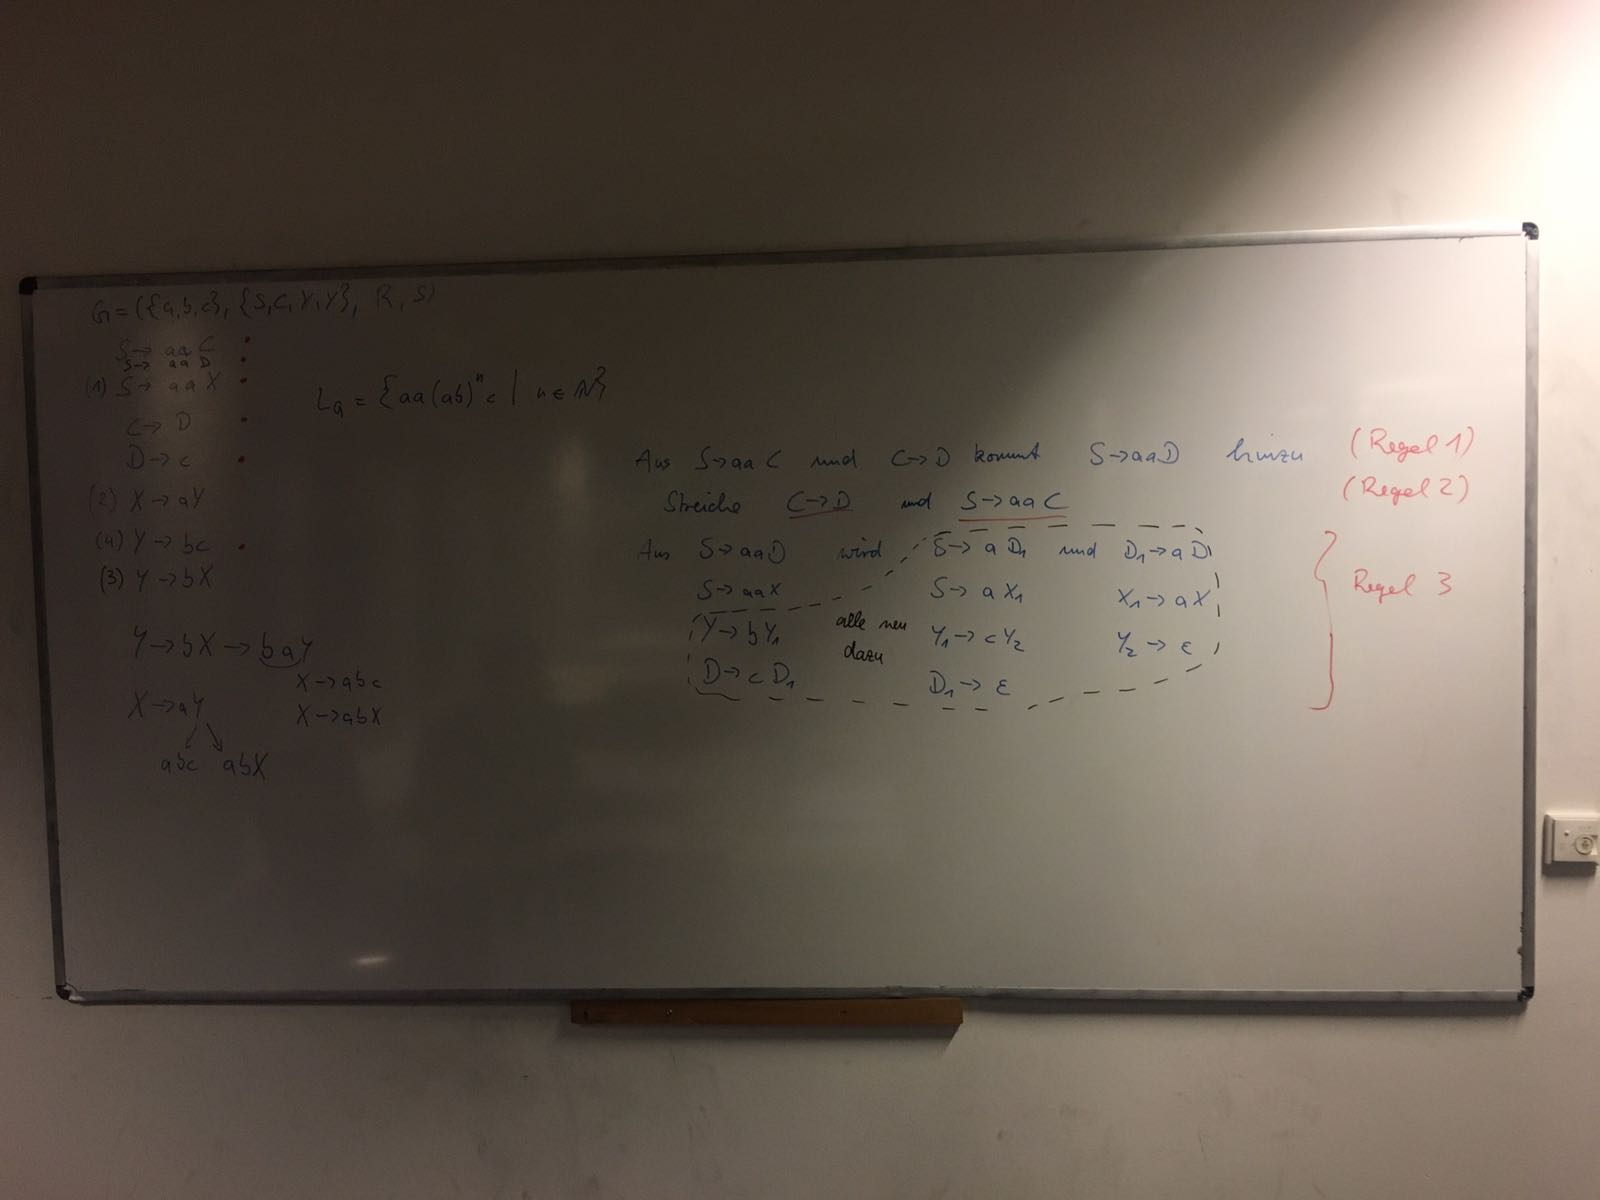
\includegraphics[width=\textwidth]{bilder/serie08_aufgabe4_1.jpg}

    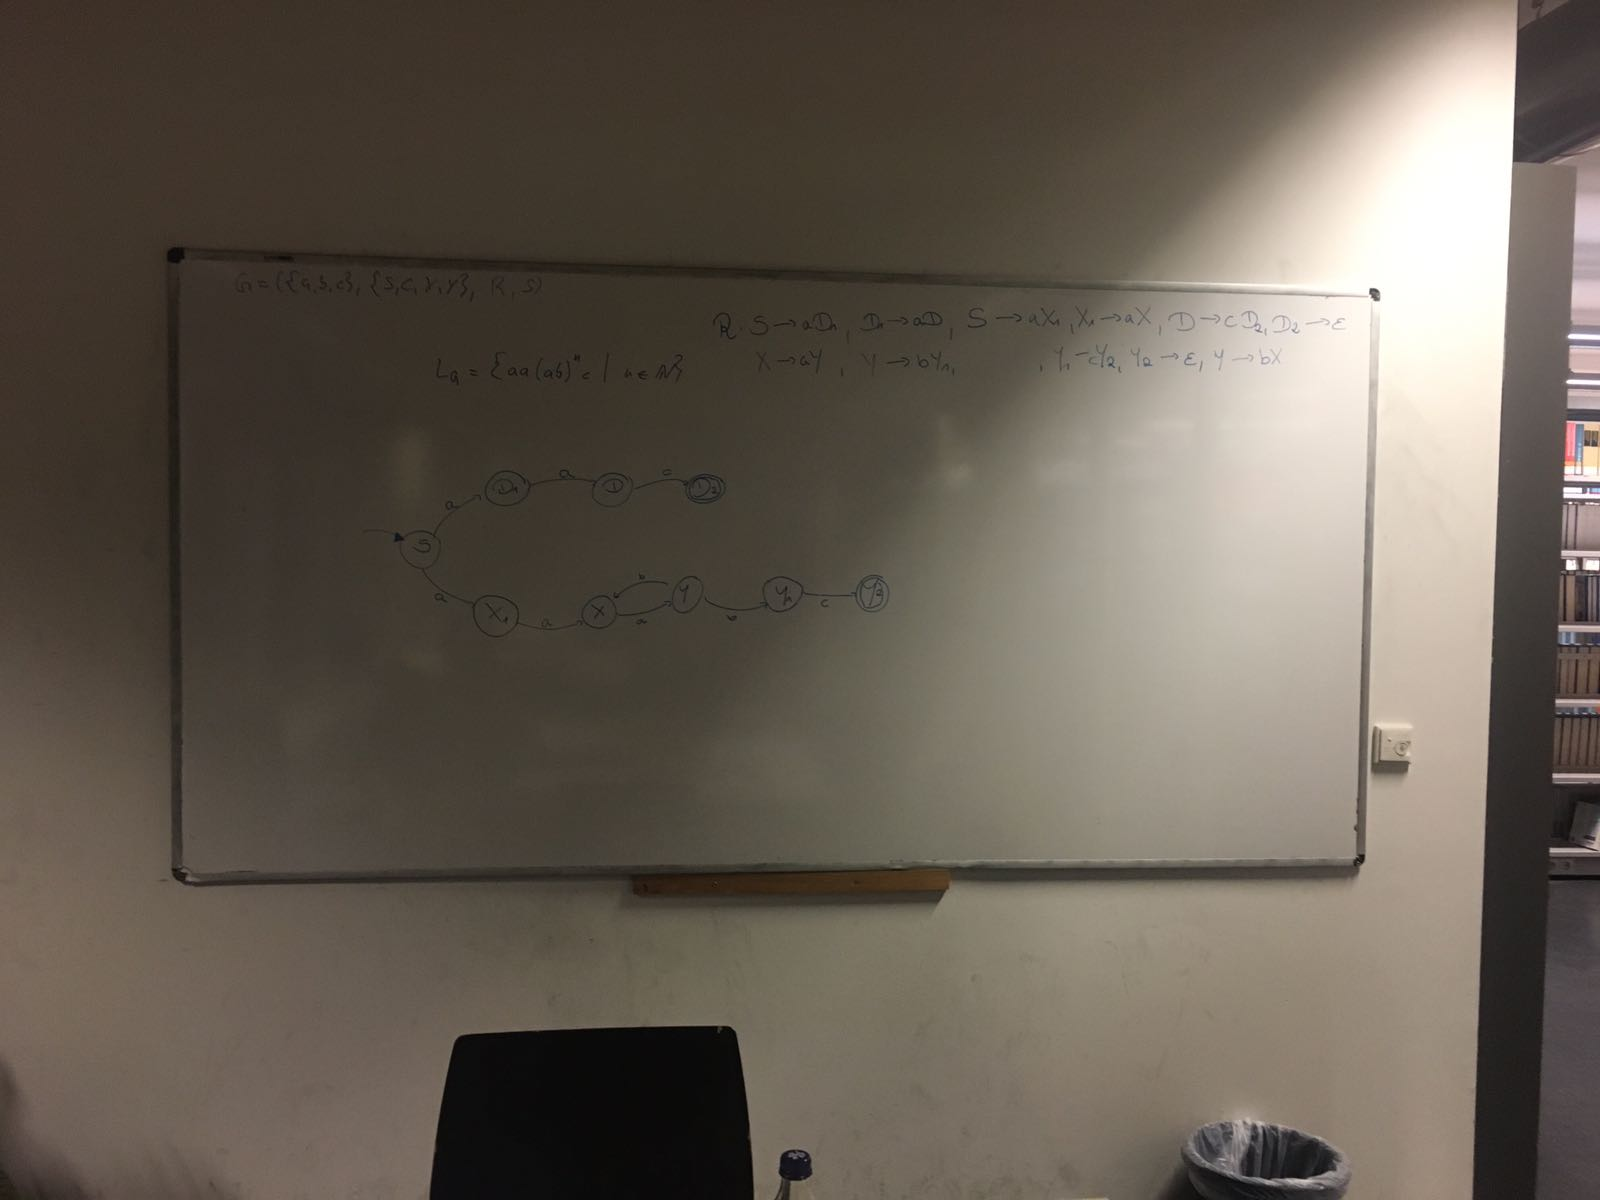
\includegraphics[width=\textwidth]{bilder/serie08_aufgabe4_2.jpg}
\end{enumerate}



\subsubsection{Serie 9}
\label{sub:serie_9}

\begin{enumerate}[1.]
  \item ---
  \item \ \\
    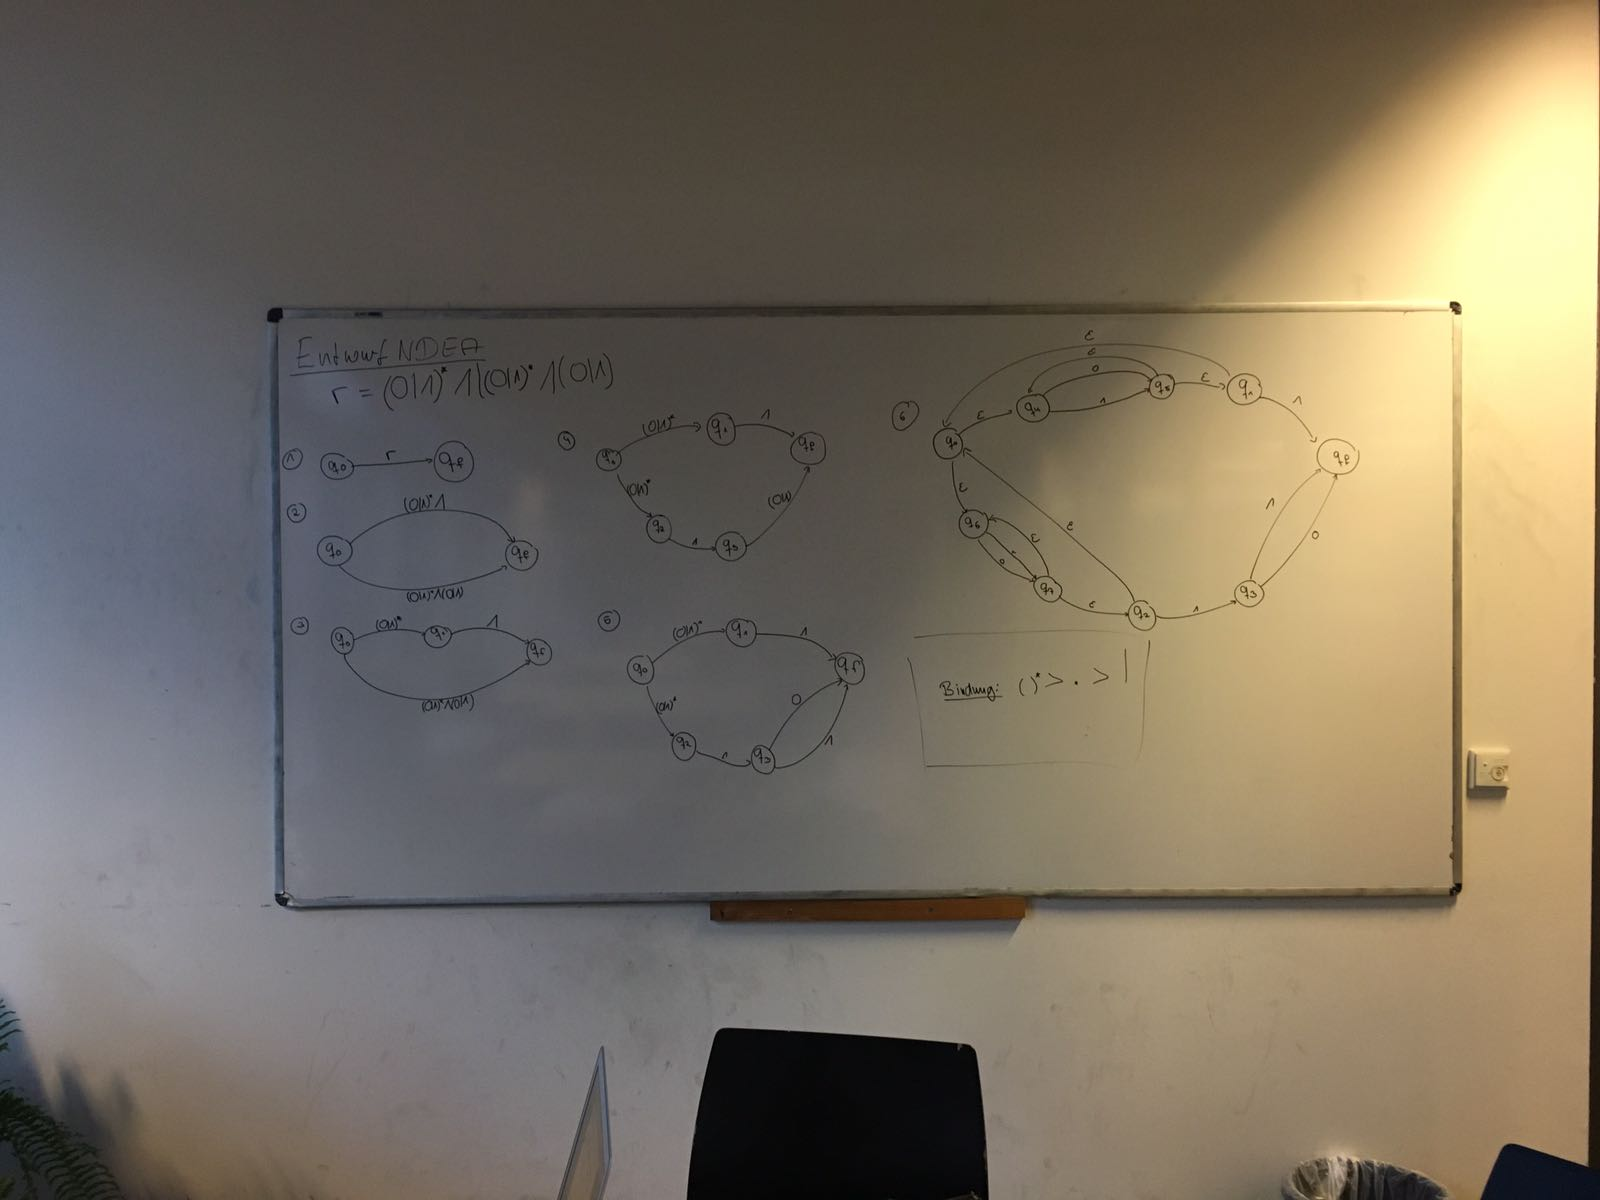
\includegraphics[width=\textwidth]{bilder/serie09_aufgabe2_1.jpg}
  \item ---
\end{enumerate}



\subsubsection{Serie 10}
\label{sub:serie_10}

\begin{enumerate}[1.]
  \item
    \begin{enumerate}
      \item A1:
        \begin{align*}
          \begin{matrix}
              & a      & b      & c      & d      & e      & f\\
            a & \times &        & \times & \times & \times & \times\\
            b &        & \times & \times & \times & \times & \times\\
            c & \times & \times & \times &        & \times & \times\\
            d & \times & \times &        & \times & \times & \times\\
            e & \times & \times & \times & \times & \times & \\
            f & \times & \times & \times & \times &        & \times
          \end{matrix}
        \end{align*}
        \begin{align*}
          [a] & = \{ a, b \}\\
          [b] & = \{ a, b \}\\
          [c] & = \{ c, d \}\\
          [d] & = \{ c, d \}\\
          [e] & = \{ e, f \}\\
          [f] & = \{ e, f \}
        \end{align*}

      \item Der Myhill-Nerode-Index beträgt $3$, da A1 genau $3$
        Äquivalenzklassen besitzt ($\{a,b\}, \{c,d\}, \{e,f\}$).

      \item \
        \begin{center}
          \begin{tikzpicture}[scale=1,node distance=0.8cm,auto]
            \node [state, initial] (ab) {$a,b$};
            \node [state, accepting] (cd) [below=of ab] {$c,d$};
            \node [state] (ef) [below=of cd] {$e,f$};

            \path[->] (ab)  edge [loop right] node {$0$}    ();
            \path[->] (ab)  edge              node {$1$}    (cd)
                      (cd)  edge              node {$0,1$}  (ef);
            \path[->] (ef)  edge [loop right] node {$0,1$}  ();
          \end{tikzpicture}
        \end{center}

      \item A2:
        \begin{align*}
          \begin{matrix}
                 & z_0    & z_1    & z_2    & z_3    & z_4    & z_5    & z_6    & z_7\\
            z_0  & \times & \times & \times & \times &        &        & \times & \times\\
            z_1  & \times & \times & \times & \times & \times & \times & \times & \times\\
            z_2  & \times & \times & \times & \times & \times & \times & \times & \\
            z_3  & \times & \times & \times & \times & \times & \times & \times & \times\\
            z_4  &        & \times & \times & \times & \times &        & \times & \times\\
            z_5  &        & \times & \times & \times &        & \times & \times & \times\\
            z_6  & \times & \times & \times & \times & \times & \times & \times & \times\\
            z_7  & \times & \times &        & \times & \times & \times & \times & \times\\
          \end{matrix}
        \end{align*}
        \begin{align*}
          [z_0] & = \{z_0, z_4, z_5\}\\
          [z_1] & = \{z_1\}\\
          [z_2] & = \{z_2, z_7\}\\
          [z_3] & = \{z_3\}\\
          [z_4] & = \{z_0, z_4, z_5\}\\
          [z_5] & = \{z_0, z_4, z_5\}\\
          [z_6] & = \{z_6\}\\
          [z_7] & = \{z_2, z_7\}
        \end{align*}

      \item A2 hat den Myhill-Nerode-Index $5$, weil es genau $5$
        Äquivalenzklassen gibt:
        \begin{align*}
          \{z_0, z_4, z_5\}, \{z_1\}, \{z_2, z_7\}, \{z_3\}, \{z_6\}
        \end{align*}

      \item \
        \begin{center}
        \begin{tikzpicture}[scale=1,node distance=0.8cm,auto]
          \node [state, initial] (045) {$z_0, z_4, z_5$};
          \node [state] (1) [below=of 045] {$z_1$};
          \node [state, accepting] (27) [below=of 1] {$z_2, z_7$};
          \node [state] (3) [below right=of 27] {$z_3$};
          \node [state] (6) [below left=of 27] {$z_6$};

          \path[->] (045) edge [loop right] node        {$1$}   ();
          \path[->] (045) edge [bend left]  node        {$0$}   (1);
          \path[->] (1)   edge [bend left]  node        {$0$}   (045)
                          edge              node        {$1$}   (27);
          \path[->] (27)  edge              node        {$0$}   (3)
                          edge [bend left]  node        {$1$}   (6);
          \path[->] (6)   edge [bend left]  node        {$1$}   (27)
                          edge [bend right] node [swap] {$0$}   (3);
          \path[->] (3)   edge [loop right] node        {$0,1$} ();
        \end{tikzpicture}
        \end{center}

      \item Ein DEA ohne totale Zustandsübergangsfunktion hat Zustände, für die
        der Übergang bei bestimmten Zeichen nicht definiert ist. Das bedeutet,
        dass keine Zustandsänderung stattfindet und der DEA in diesem Zustand
        bleibt.

        Das heißt, dass man einen DEA ohne totale Zustandsübergangsfunktion zu
        einen mit totaler Zustandsübergangsfunktion erweitern kann, indem man
        zusätzliche Schleifen hinzufügt.

        Diesen DEA kann man dann ganz normal minimieren.
    \end{enumerate}

  \item
    \begin{enumerate}
      \item \
        \begin{center}
        \begin{tikzpicture}[scale=1, node distance=1cm, auto]
          \node [state, initial] (q_0) {$q_0$};
          \node [state] (q_1) [below right=of q_0] {$q_1$};
          \node [state] (q_3) [below left=of q_0] {$q_3$};
          \node [state, accepting] (q_2) [below left=of q_1] {$q_2$};

          \path[->] (q_0) edge node {$a$} (q_1)
                          edge node [swap] {$b$} (q_3)
                    (q_1) edge node {$a$} (q_3)
                          edge node {$b$} (q_2)
                    (q_3) edge [loop left] node {$a,b$} ()
                    (q_2) edge [loop below] node {$a,b$} ();
        \end{tikzpicture}
        \end{center}
      \item $L(A) = \{abw \mid w \in \{a, b\}^*\}$

      \item Da sich der Automat nicht weiter minimieren lässt, ist die minimale
        Pumpingzahl der Sprache gleich der Anzahl der Zustände des Automats und
        damit $4$.
      
    \end{enumerate}

\end{enumerate}


\subsection{Semantik}
\label{sec:semantik}

\subsubsection{Übung 243}
\label{ssub:Uebung 243}

Das Ersetzungs-System ist
\begin{itemize}
  \item nicht terminierend
  \item nicht beschränkt
  \item konfluent $\Rightarrow$ semi-konfluent $\Rightarrow$ lokal konfluent
  \item nicht normalisierend
  \item nicht konvergent
\end{itemize}

Der irreflexive Kern ist
\begin{itemize}
  \item terminierend
  \item nicht beschränkt
  \item konfluent $\Rightarrow$ semi-konfluent $\Rightarrow$ lokal konfluent
  \item normalisierend
  \item konvergent (weil es konfluent und terminierend ist)
\end{itemize}

\begin{thebibliography}{9}

\bibitem{hopcroft2011}
  Hopcroft, John E., Rajeev Motwani, and Jeffrey D. Ullman,
  \emph{Einführung in Automatentheorie, Formale Sprachen und Berechenbarkeit},
  Pearson Deutschland GmbH,
  2011.

\end{thebibliography}

\end{document}
